%  LaTeX support: latex@mdpi.com 
%  In case you need support, please attach all files that are necessary for compiling as well as the log file, and specify the details of your LaTeX setup (which operating system and LaTeX version / tools you are using).

% You need to save the "mdpi.cls" and "mdpi.bst" files into the same folder as this template file.

%=================================================================
\documentclass[publications,article,submit,moreauthors,pdftex,10pt,a4paper]{Definitions/mdpi} 


\usepackage{url}
\usepackage{hyperref}

\usepackage{color}
\usepackage{fancyvrb}
\newcommand{\VerbBar}{|}
\newcommand{\VERB}{\Verb[commandchars=\\\{\}]}
\DefineVerbatimEnvironment{Highlighting}{Verbatim}{commandchars=\\\{\}}
% Add ',fontsize=\small' for more characters per line
\usepackage{framed}
\definecolor{shadecolor}{RGB}{248,248,248}
\newenvironment{Shaded}{\begin{snugshade}}{\end{snugshade}}
\newcommand{\AlertTok}[1]{\textcolor[rgb]{0.94,0.16,0.16}{#1}}
\newcommand{\AnnotationTok}[1]{\textcolor[rgb]{0.56,0.35,0.01}{\textbf{\textit{#1}}}}
\newcommand{\AttributeTok}[1]{\textcolor[rgb]{0.77,0.63,0.00}{#1}}
\newcommand{\BaseNTok}[1]{\textcolor[rgb]{0.00,0.00,0.81}{#1}}
\newcommand{\BuiltInTok}[1]{#1}
\newcommand{\CharTok}[1]{\textcolor[rgb]{0.31,0.60,0.02}{#1}}
\newcommand{\CommentTok}[1]{\textcolor[rgb]{0.56,0.35,0.01}{\textit{#1}}}
\newcommand{\CommentVarTok}[1]{\textcolor[rgb]{0.56,0.35,0.01}{\textbf{\textit{#1}}}}
\newcommand{\ConstantTok}[1]{\textcolor[rgb]{0.00,0.00,0.00}{#1}}
\newcommand{\ControlFlowTok}[1]{\textcolor[rgb]{0.13,0.29,0.53}{\textbf{#1}}}
\newcommand{\DataTypeTok}[1]{\textcolor[rgb]{0.13,0.29,0.53}{#1}}
\newcommand{\DecValTok}[1]{\textcolor[rgb]{0.00,0.00,0.81}{#1}}
\newcommand{\DocumentationTok}[1]{\textcolor[rgb]{0.56,0.35,0.01}{\textbf{\textit{#1}}}}
\newcommand{\ErrorTok}[1]{\textcolor[rgb]{0.64,0.00,0.00}{\textbf{#1}}}
\newcommand{\ExtensionTok}[1]{#1}
\newcommand{\FloatTok}[1]{\textcolor[rgb]{0.00,0.00,0.81}{#1}}
\newcommand{\FunctionTok}[1]{\textcolor[rgb]{0.00,0.00,0.00}{#1}}
\newcommand{\ImportTok}[1]{#1}
\newcommand{\InformationTok}[1]{\textcolor[rgb]{0.56,0.35,0.01}{\textbf{\textit{#1}}}}
\newcommand{\KeywordTok}[1]{\textcolor[rgb]{0.13,0.29,0.53}{\textbf{#1}}}
\newcommand{\NormalTok}[1]{#1}
\newcommand{\OperatorTok}[1]{\textcolor[rgb]{0.81,0.36,0.00}{\textbf{#1}}}
\newcommand{\OtherTok}[1]{\textcolor[rgb]{0.56,0.35,0.01}{#1}}
\newcommand{\PreprocessorTok}[1]{\textcolor[rgb]{0.56,0.35,0.01}{\textit{#1}}}
\newcommand{\RegionMarkerTok}[1]{#1}
\newcommand{\SpecialCharTok}[1]{\textcolor[rgb]{0.00,0.00,0.00}{#1}}
\newcommand{\SpecialStringTok}[1]{\textcolor[rgb]{0.31,0.60,0.02}{#1}}
\newcommand{\StringTok}[1]{\textcolor[rgb]{0.31,0.60,0.02}{#1}}
\newcommand{\VariableTok}[1]{\textcolor[rgb]{0.00,0.00,0.00}{#1}}
\newcommand{\VerbatimStringTok}[1]{\textcolor[rgb]{0.31,0.60,0.02}{#1}}
\newcommand{\WarningTok}[1]{\textcolor[rgb]{0.56,0.35,0.01}{\textbf{\textit{#1}}}}
\usepackage{graphicx,grffile}
\makeatletter
\def\maxwidth{\ifdim\Gin@nat@width>\linewidth\linewidth\else\Gin@nat@width\fi}
\def\maxheight{\ifdim\Gin@nat@height>\textheight\textheight\else\Gin@nat@height\fi}
\makeatother
% Scale images if necessary, so that they will not overflow the page
% margins by default, and it is still possible to overwrite the defaults
% using explicit options in \includegraphics[width, height, ...]{}
\setkeys{Gin}{width=\maxwidth,height=\maxheight,keepaspectratio}
\IfFileExists{parskip.sty}{%
\usepackage{parskip}
}{% else
\setlength{\parindent}{0pt}
\setlength{\parskip}{6pt plus 2pt minus 1pt}
}
\setlength{\emergencystretch}{3em}  % prevent overfull lines
\providecommand{\tightlist}{%
  \setlength{\itemsep}{0pt}\setlength{\parskip}{0pt}}
\setcounter{secnumdepth}{0}
% Redefines (sub)paragraphs to behave more like sections
\ifx\paragraph\undefined\else
\let\oldparagraph\paragraph
\renewcommand{\paragraph}[1]{\oldparagraph{#1}\mbox{}}
\fi
\ifx\subparagraph\undefined\else
\let\oldsubparagraph\subparagraph
\renewcommand{\subparagraph}[1]{\oldsubparagraph{#1}\mbox{}}
\fi

% If you would like to post an early version of this manuscript as a preprint, you may use preprint as the journal and change 'submit' to 'accept'. The document class line would be, e.g., \documentclass[preprints,article,accept,moreauthors,pdftex,10pt,a4paper]{mdpi}. This is especially recommended for submission to arXiv, where line numbers should be removed before posting. For preprints.org, the editorial staff will make this change immediately prior to posting.

%
%--------------------
% Class Options:
%--------------------
% journal
%----------
% Choose between the following MDPI journals:
% acoustics, actuators, addictions, admsci, aerospace, agriculture, agronomy, algorithms, animals, antibiotics, antibodies, antioxidants, applsci, arts, asi, atmosphere, atoms, axioms, batteries, bdcc, behavsci, beverages, bioengineering, biology, biomedicines, biomimetics, biomolecules, biosensors, brainsci, buildings, carbon, cancers, catalysts, cells, ceramics, challenges, chemengineering, chemosensors, children, cleantechnol, climate, clockssleep, cmd, coatings, colloids, computation, computers, condensedmatter, cosmetics, cryptography, crystals, cybersecurity, data, dentistry, designs, diagnostics, dairy, diseases, diversity, drones, econometrics, economies, education, electrochem, electrochemistry, electronics, energies, entropy, environments, epigenomes, est, fermentation, fibers, fire, fishes, fluids, foods, forecasting, forests, fractalfract, futureinternet, galaxies, games, gastrointestdisord, gels, genealogy, genes, geohazards, geosciences, geriatrics, hazardousmatters, healthcare, heritage, highthroughput, horticulturae, humanities, hydrology, informatics, information, infrastructures, inorganics, insects, instruments, ijerph, ijfs, ijms, ijgi, ijtpp, inventions, j, jcdd, jcm, jcs, jdb, jfb, jfmk, jimaging, jof, jintelligence, jlpea, jmmp, jmse, jpm, jrfm, jsan, land, languages, laws, life, literature, logistics, lubricants, machines, magnetochemistry, make, marinedrugs, materials, mathematics, mca, medsci, medicina, medicines, membranes, metabolites, metals, microarrays, micromachines, microorganisms, minerals, modelling, molbank, molecules, mps, mti, nanomaterials, ncrna, neonatalscreening, neuroglia, nitrogen, nutrients, ohbm, particles, pathogens, pharmaceuticals, pharmaceutics, pharmacy, philosophies, photonics, plants, plasma, polymers, polysaccharides, proceedings, processes, proteomes, publications, quaternary, qubs, reactions, recycling, religions, remotesensing, reports, resources, risks, robotics, safety, sci, scipharm, sensors, separations, sexes, sinusitis, smartcities, socsci, societies, soilsystems, sports, standards, stats, surfaces, surgeries, sustainability, symmetry, systems, technologies, toxics, toxins, tropicalmed, universe, urbansci, vaccines, vehicles, vetsci, vibration, viruses, vision, water, wem, wevj
%---------
% article
%---------
% The default type of manuscript is article, but can be replaced by: 
% abstract, addendum, article, benchmark, book, bookreview, briefreport, casereport, changes, comment, commentary, communication, conceptpaper, correction, conferenceproceedings, conferencereport, expressionofconcern, extendedabstract, meetingreport, creative, datadescriptor, discussion, editorial, essay, erratum, hypothesis, interestingimages, letter, meetingreport, newbookreceived, opinion, obituary, projectreport, reply, reprint, retraction, review, perspective, protocol, shortnote, supfile, technicalnote, viewpoint
% supfile = supplementary materials
% protocol: If you are preparing a "Protocol" paper, please refer to http://www.mdpi.com/journal/mps/instructions for details on its expected structure and content.
%----------
% submit
%----------
% The class option "submit" will be changed to "accept" by the Editorial Office when the paper is accepted. This will only make changes to the frontpage (e.g., the logo of the journal will get visible), the headings, and the copyright information. Also, line numbering will be removed. Journal info and pagination for accepted papers will also be assigned by the Editorial Office.
%------------------
% moreauthors
%------------------
% If there is only one author the class option oneauthor should be used. Otherwise use the class option moreauthors.
%---------
% pdftex
%---------
% The option pdftex is for use with pdfLaTeX. If eps figures are used, remove the option pdftex and use LaTeX and dvi2pdf.

%=================================================================
\firstpage{1} 
\makeatletter 
\setcounter{page}{\@firstpage} 
\makeatother
\pubvolume{xx}
\issuenum{1}
\articlenumber{5}
\pubyear{2019}
\copyrightyear{2019}
%\externaleditor{Academic Editor: name}
\history{Received: date; Accepted: date; Published: date}
%\updates{yes} % If there is an update available, un-comment this line

%% MDPI internal command: uncomment if new journal that already uses continuous page numbers 
%\continuouspages{yes}

%------------------------------------------------------------------
% The following line should be uncommented if the LaTeX file is uploaded to arXiv.org
%\pdfoutput=1

%=================================================================
% Add packages and commands here. The following packages are loaded in our class file: fontenc, calc, indentfirst, fancyhdr, graphicx, lastpage, ifthen, lineno, float, amsmath, setspace, enumitem, mathpazo, booktabs, titlesec, etoolbox, amsthm, hyphenat, natbib, hyperref, footmisc, geometry, caption, url, mdframed, tabto, soul, multirow, microtype, tikz

%=================================================================
%% Please use the following mathematics environments: Theorem, Lemma, Corollary, Proposition, Characterization, Property, Problem, Example, ExamplesandDefinitions, Hypothesis, Remark, Definition
%% For proofs, please use the proof environment (the amsthm package is loaded by the MDPI class).

%=================================================================
% Full title of the paper (Capitalized)
\Title{Verified, shared, modular, and provenance based research communication with the Dat protocol}

% Author Orchid ID: enter ID or remove command
\newcommand{\orcidauthorA}{0000-0003-1050-6809} % Add \orcidA{} behind the author's name
%\newcommand{\orcidauthorB}{0000-0000-000-000X} % Add \orcidB{} behind the author's name

% Authors, for the paper (add full first names)
\Author{Chris Hartgerink$^{1}$\orcidA{}}

% Authors, for metadata in PDF
\AuthorNames{Chris Hartgerink}

% Affiliations / Addresses (Add [1] after \address if there is only one affiliation.)
\address{%
$^{1}$ \quad Independent researcher; chris@libscie.org}

% Contact information of the corresponding author
\corres{Correspondence: chris@libscie.org}

% Current address and/or shared authorship
% \firstnote{Current address: Affiliation 3} 
% \secondnote{These authors contributed equally to this work.}
% The commands \thirdnote{} till \eighthnote{} are available for further notes

%\simplesumm{} % Simple summary

%\conference{} % An extended version of a conference paper

% Abstract (Do not insert blank lines, i.e. \\) 
\abstract{A scholarly communication system needs to register, distribute,
certify, archive, and incentivize knowledge production. The current
article-based system technically fulfills these functions, but
suboptimally. I propose a module-based communication infrastructure
that attempts to take a wider view of these functions and optimize the
fulfillment of the five functions of scholarly
communication. Scholarly modules are conceptualized as the constituent
parts of a research process as determined by a researcher. These can
be text, but also code, data, and any other relevant piece of
information. The chronology of these modules is registered by
iteratively linking to each other, creating a provenance record of
parent- and child modules (and a network of modules). These scholarly
modules are linked to scholarly profiles, creating a network of
profiles, and a network of how profiles relate to their constituent
modules. All these scholarly modules would be communicated on the new
peer-to-peer Web protocol Dat (https://datproject.org), which provides a
decentralized register that is immutable, facilitates greater content
integrity than the current system through verification, and is
open-by-design. open-by-design would also allow diversity in the way
content is consumed, discovered, and evaluated to arise. This initial
proposal needs to be refined and developed further based on technical
developments of the Dat protocol and its implementations, and
discussions within the scholarly community to evaluate the qualities
claimed here. Nonetheless, a minimal prototype is available today and
this is technically feasible.}

% Keywords
\keyword{metaresearch; decentralization; decentralisation; publishing; p2p}

% The fields PACS, MSC, and JEL may be left empty or commented out if not applicable
%\PACS{J0101}
%\MSC{}
%\JEL{}

%%%%%%%%%%%%%%%%%%%%%%%%%%%%%%%%%%%%%%%%%%
% Only for the journal Diversity
%\LSID{\url{http://}}

%%%%%%%%%%%%%%%%%%%%%%%%%%%%%%%%%%%%%%%%%%
% Only for the journal Applied Sciences:
%\featuredapplication{Authors are encouraged to provide a concise description of the specific application or a potential application of the work. This section is not mandatory.}
%%%%%%%%%%%%%%%%%%%%%%%%%%%%%%%%%%%%%%%%%%

%%%%%%%%%%%%%%%%%%%%%%%%%%%%%%%%%%%%%%%%%%
% Only for the journal Data:
%\dataset{DOI number or link to the deposited data set in cases where the data set is published or set to be published separately. If the data set is submitted and will be published as a supplement to this paper in the journal Data, this field will be filled by the editors of the journal. In this case, please make sure to submit the data set as a supplement when entering your manuscript into our manuscript editorial system.}

%\datasetlicense{license under which the data set is made available (CC0, CC-BY, CC-BY-SA, CC-BY-NC, etc.)}

%%%%%%%%%%%%%%%%%%%%%%%%%%%%%%%%%%%%%%%%%%
% Only for the journal Toxins
%\keycontribution{The breakthroughs or highlights of the manuscript. Authors can write one or two sentences to describe the most important part of the paper.}

%\setcounter{secnumdepth}{4}
%%%%%%%%%%%%%%%%%%%%%%%%%%%%%%%%%%%%%%%%%%
\begin{document}
%%%%%%%%%%%%%%%%%%%%%%%%%%%%%%%%%%%%%%%%%%
%% Only for the journal Gels: Please place the Experimental Section after the Conclusions

\section*{Introduction}

In scholarly research, communication needs to be thorough and
parsimonious in logging the order of various research steps, while at
the same time being functional in seeking- and distributing knowledge.
Roosendaal and Geurts proposed that any scholarly communication system
needs to serve as a (1) registration-, (2) certification-, (3)
awareness-, and (4) archival system \citep{roosendaal1998}. Sompel
and colleagues added that it also needs to serve as an (5) incentive
system \citep{doi:10.1045/september2004-vandesompel}.

How the functions of scholarly communication are conceptualized and
implemented directly impact (the effectiveness of) scholarly research.
For example, an incentive system might be present where number of
publications or publication outlet is more important than the quality of
the publications \citep{doi:10.3389/fnhum.2018.00037}. In a narrow sense, this scholarly
communication system serves the fifth function of providing an incentive
system. In a wider sense, it undermines the goal of scholarly research,
which scholarly communication is a part of, and therefore does not serve
its purpose.

Narrow conceptualizations of the functions of a scholarly
communication system can be identified in the current article-based
system.  Registration occurs for published works, but registration is
incomplete due to selective publication 
\citep[e.g., 1 out of 2 registered
clinical trials gets published;][]{doi:10.1016/0140-6736_91_90201-y} making research highly
inefficient \citep{doi:10.1371/journal.pone.0084896}. Certification
occurs through peer review \citep{doi:10.1038/nature05008} but peer
review is confounded by a set of human biases at the reporting- and
evaluation stages \citep[e.g., methods are evaluated as of higher quality
when they result in statistically significant results than when in
statistically nonsignificant results;][]{doi:10.1007/bf01173636}. Awareness occurs, but increasingly so
for only those researchers with the financial means to access or make
accessible.  Restrictions on the sharing of scholarly information
hampers discovery and widespread dissemination. Content is archived,
but is centralized (i.e., failure prone), separated from the main
dissemination infrastructure, and not available until an arbitrary
trigger event occurs \citep[i.e., a dark archive;][]{doi:10.1629/uksg.215}.

The scholarly paper seems an anachronistic form of communication in
light of how we now know it undermines the functions it is supposed to
serve. When no alternative communication form was feasible (i.e.,
before the Internet and the Web), the scholarly paper seemed a
reasonable and balanced form for communication. However, already in
1998, seven years after the first Web browser was released,
researchers associated with the scholarly publisher Elsevier suggested
to make changes to the way scholars communicate scholarly research
\citep{doi:10.1108/eum0000000007185}. More specifically, they suggested to
change the communication to a more modular form, which would help
iterate research more frequently and increase feedback moments \citep[high
speed of feedback was essential to for example Nature's rise during
the early twentieth century;][]{isbn:9780226261454}. Throughout the
years, others also suggested various perspectives on modularity
\citep{doi:10.3389/fncom.2012.00019,doi:10.7717/peerj-cs.78} and
suggested micro- and nanopublications \citep{doi:10.7717/peerj-cs.78,
doi:10.1186/2041-1480-5-28}.

Modular scholarly outputs, each a separate step in the research
process, could supplement the scholarly article \citep[as detailed in][]{doi:10.3390/publications6020021}. Scholarly textbooks \citep[i.e.,
vademecum science;][]{isbn:9780226253251} communicate findings with few
details and a high degree of certainty; scholarly articles present
relatively more details and less certainty than textbooks, but still
lack the detail to reproduce results. This lack of detail is
multiplied by the increasingly complex research pipelines due to
technological changes and the size of data processed. Moreover,
textbooks and articles construct narratives across findings because
they report far after events have happened. Scholarly modules could
serve as a base for scholarly articles, reporting more details, less
certainty of findings, and where events are reported closer to their
occurrence. Granular reporting could facilitate reproducibility (i.e.,
it is easier to reproduce one action with more details than multiple
actions with fewer details per action); earlier reporting could
facilitate discussion by making it practical for the research process
\citep[extending the idea of Registered Reports;][]{doi:10.1016/j.cortex.2012.12.016} and making content easier to find
and reuse. As findings become replicated and more consensus about a
finding starts to arise, findings could move up the 'chain' and be
integrated into scholarly articles and textbooks. Articles and books
would then provide overviews and larger narratives to understand
historical developments within scholarly research. Figure
\ref{fig:datcom-fig1} provides a conceptual depiction of how these
different forms of documenting findings relate to each other.

\begin{figure}
{\centering 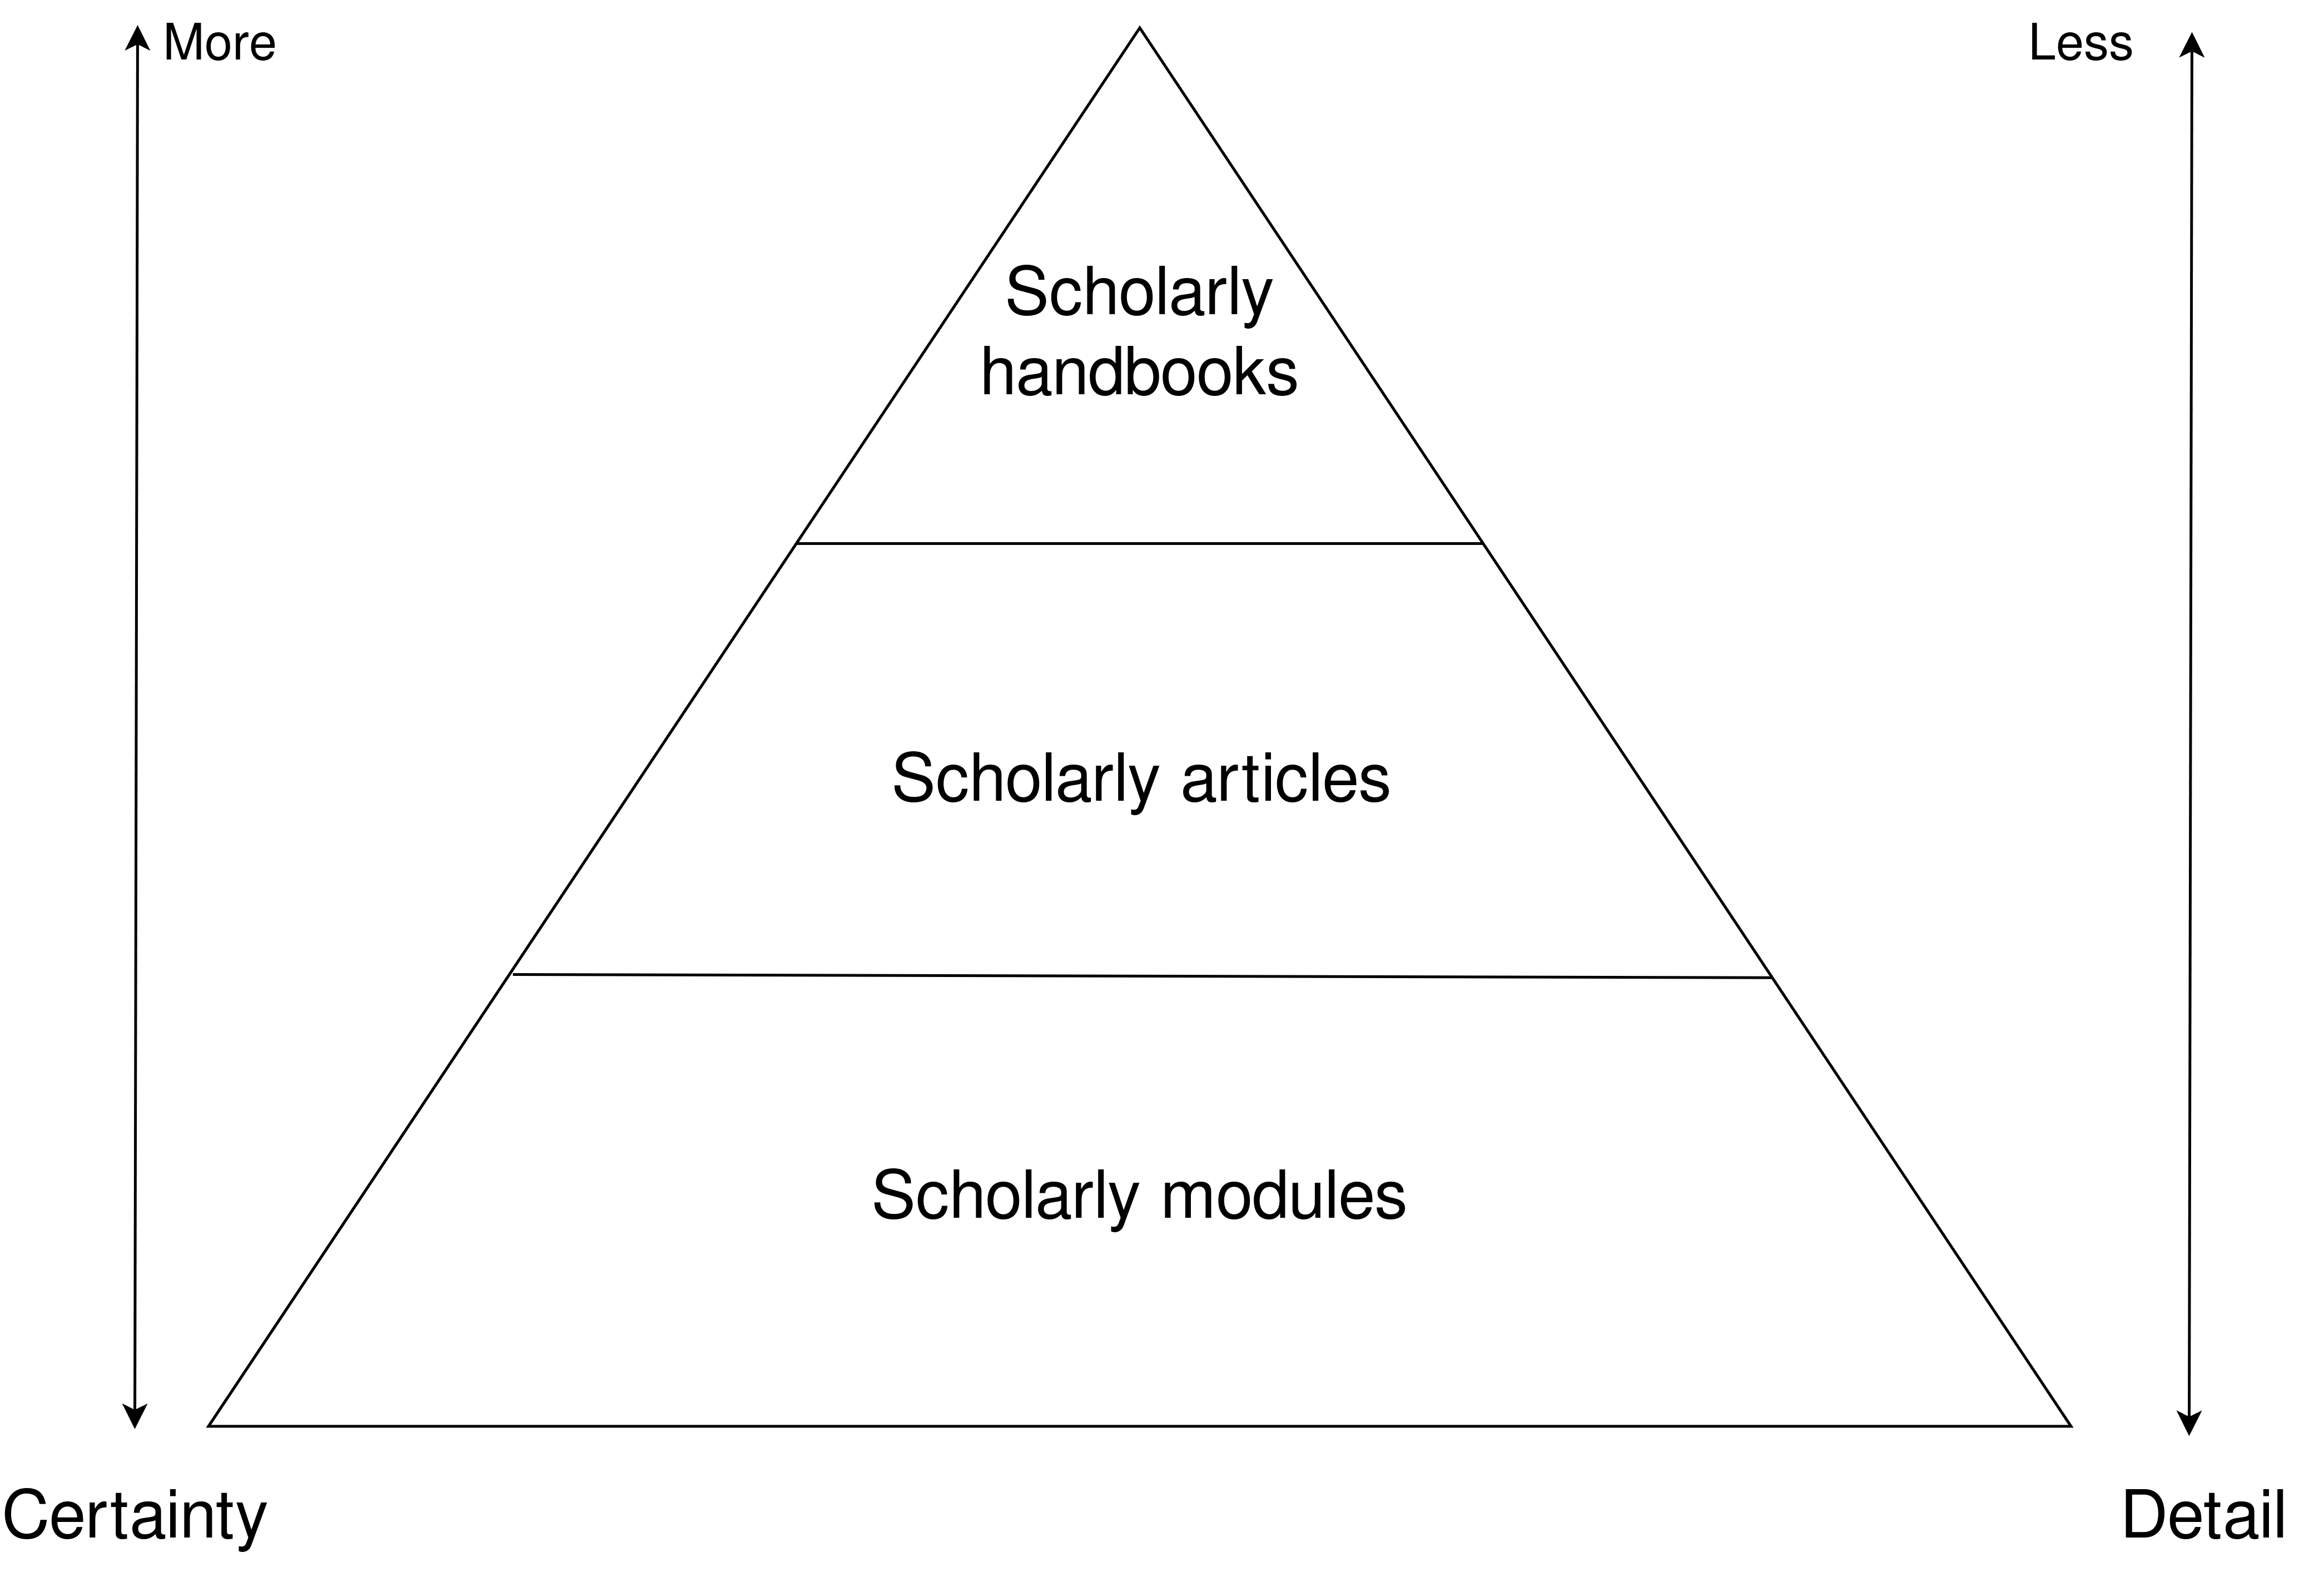
\includegraphics[width=1\linewidth]{fig1}}
\caption{Conceptual depiction of how different forms of scholarly communication relate to each other in both detail and certainty.}
\label{fig:datcom-fig1}
\end{figure}

Below I extend on technical details for a modular scholarly communication infrastructure that facilitates (more) continuous communication and builds on recent advances in Web infrastructures. The premise of this scholarly infrastructure is a wider interpretation of the five functions of a scholarly communication system, where (1) registration is (more) complete, (2) certification occurs by embedding chronology to prevent misrepresentation and by increased potential for verification and peer discussion, (3) unrestricted awareness (i.e., access) is embedded in the underlying peer-to-peer protocol that locks it open-by-design, (4) archival is facilitated by simplified copying, and (5) making more specific scholarly evaluation possible to improve incentives \citep[for an initial proposal of such evaluation systems see][]{doi:10.3390/publications6020021}. First, I expand on the functionality of the Internet protocol \href{https://datproject.org}{Dat} and how it facilitates improved dissemination and archival. Second, I illustrate an initial design of modular scholarly communication using this protocol to facilitate better registration and certification. 

\section*{Dat protocol}\label{dat-protocol}

The Dat protocol (\texttt{dat://}) is a peer-to-peer protocol, with
persistent public keys per filesystem \citep{doi:10.31219/osf.io/nsv2c}. Each filesystem is a
folder that lives on the Dat network. Upon creation, each Dat filesystem
receives a unique 64 character hash address, which provides read-only
access to anyone who has knowledge of the hash. Below an example
filesystem is presented. Each Dat filesystem has a persistent public
key, which is unaffected by bit-level changes within it (e.g., when a
file is modified or created). Other peer-to-peer protocols, such as
BitTorrent or the Inter Planetary File System (IPFS), receive new public
keys upon bit-level changes in the filesystem and require re-sharing
those keys after each change.

\begin{Shaded}
\begin{Highlighting}[]
\ExtensionTok{0c6...613/}
\KeywordTok{|}\ExtensionTok{---}\NormalTok{ file1}
\KeywordTok{|}\ExtensionTok{---}\NormalTok{ file2}
\KeywordTok{|}\ExtensionTok{---}\NormalTok{ file3}
\KeywordTok{|}\ExtensionTok{---}\NormalTok{ file4}
\end{Highlighting}
\end{Shaded}

Bit-level changes within a Dat filesystem are verified with cryptographically signed hashes of the changes in a Merkle Tree. In effect, using a Merkle Tree creates a verified append-only register. In a Merkle Tree, contents are decomposed into chunks that are subsequently hashed in a tree (as illustrated in Figure \ref{fig:datcom-fig2}), adding each new action to the tree at the lowest level. These hashes are cryptographically signed with the permitted users' private keys. The Dat protocol regards all actions in its filesystem as  \texttt{put} or
\texttt{del} commands to the filesystem, allowing all operations on the
filesystem to be regarded as actions append to a register (i.e., log).
For example, if an empty \texttt{file5} was added to the Dat filesystem
presented above, the register would include
\texttt{{[}put{]}\ /file5\ 0\ B\ (0\ blocks)}; if we delete the file, it
would log \texttt{{[}del{]}\ /file5}. The complete register for this Dat
filesystem is as follows

\begin{figure}[!h]

{\centering 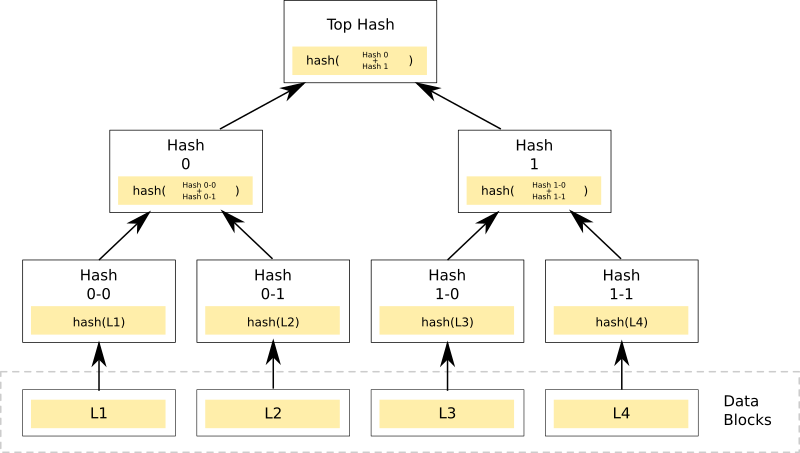
\includegraphics[width=1\linewidth]{Hash_Tree.svg} 

}

\caption{A diagram depicting how a Merkle Tree hashes initial chunks of information into one top hash, with which the content can be verified.}\label{fig:datcom-fig2}
\end{figure}


\begin{Shaded}
\begin{Highlighting}[]
\ExtensionTok{dat}\NormalTok{://0c6...613}

\ExtensionTok{1}\NormalTok{ [put] /file1 0 B (0 blocks)}
\ExtensionTok{2}\NormalTok{ [put] /file2 0 B (0 blocks)}
\ExtensionTok{3}\NormalTok{ [put] /file3 0 B (0 blocks)}
\ExtensionTok{4}\NormalTok{ [put] /file4 0 B (0 blocks)}
\ExtensionTok{5}\NormalTok{ [put] /file5 0 B (0 blocks)}
\ExtensionTok{6}\NormalTok{ [del] /file5}
\end{Highlighting}
\end{Shaded}

The persistent public key combined with the append-only register,
results in persistent versioned addresses for filesystems that also
ensure content integrity. For example, based on the register presented
above, we see that version 5 includes \texttt{file5} whereas version 6
does not. By appending \texttt{+5} to the public key
(\texttt{dat://0c66...613+5}) we can view the Dat filesystem as it
existed at version 5 and be ensured that the contents we receive are the
exact contents at that version. If the specific Dat filesystem is
available from at least one peer on the network, it means that both
`link rot' and `content drift' \citep{doi:10.1371/journal.pone.0115253, doi:10.1371/journal.pone.0167475}
could become superfluous.

Any content posted to the Dat protocol is as publicly available as the public key of that Dat filesystem is shared. More specifically, the Dat protocol is inherently open. As such, if that key is widely shared, the content will also be harder or impossible to remove from the network because other peers (can) have copied it. Conversely, if that key is shared among just few people that content can more easily disappear from the network but remains more private. This is important in light of privacy issues, because researchers cannot unshare personal data after they have widely broadcasted it. However, because the Dat protocol is a peer-to-peer protocol and users connect directly to each other, information is not mediated. The protocol uses package encryption by default which can also help improve secure and private transfers of (sensitive) data. Users would (most likely) also remain personally responsible for the information they (wrongly) disclose on the network.

\section*{Verified modular scholarly
communication}\label{verified-modular-scholarly-communication}

Here I propose an initial technical design of verified modular scholarly communication using the Dat protocol. Scholarly modules are instantiated as separate Dat filesystems for each researcher or for each module of scholarly content. Scholarly content could entail virtually anything the researcher wants or needs to communicate in order to verify findings \citep[see also ][]{doi:10.3390/publications6020021}. Hence, there is no restriction to text as it is in the current article-based scholarly communication system; it may also include photographs, data files, scripts, etc. Note that all presented hypothetical scenarios next include shortened Dat links and the unshortened links can be found in the Supporting Information.

\subsection*{Scholarly profiles}\label{scholarly-profiles}

Before communicating research modules, a researcher would need to have a
place to broadcast that information. Increasingly, researchers are
acquiring centralized scholarly profiles to identify the work they do,
such as ORCIDs, ResearcherIDs, Google Scholar profiles, or ResearchGate
profiles. A decentralized scholarly profile in a Dat filesystem is
similar and provides a unique ID (i.e., public key) for each researcher.
However, researchers can modify their profiles freely because they
retain full ownership and control of their data (as opposed to
centralized profiles) and are not tied to one platform. As such, with
decentralized scholarly profiles on the Dat network, the researcher
permits others access to their profile instead of a service permitting
them to have a profile.

Each Dat filesystem is initialized with a \texttt{dat.json} with some
initial metadata, including its own Dat public key, the title (i.e.,
name) of the filesystem and a description. For example, Alice wants to
create a scholarly profile and initializes her Dat filesystem, resulting
in:

\begin{Shaded}
\begin{Highlighting}[]
\FunctionTok{\{}
  \DataTypeTok{"title"}\FunctionTok{:} \StringTok{"Alice"}\FunctionTok{,}
  \DataTypeTok{"description"}\FunctionTok{:} \StringTok{"I am a physicist at CERN-LHC. As a fan of the }
  \StringTok{decentralized Web, I look forward to communicating my research in }
  \StringTok{a digital native manner and in a way that is not limited to just text."}
  \StringTok{text."}\FunctionTok{,}
  \DataTypeTok{"url"}\FunctionTok{:} \StringTok{"dat://b49...551"}
\FunctionTok{\}}
\end{Highlighting}
\end{Shaded}

Because \texttt{dat.json} is a generic container for metadata across the
Dat network, I propose adding \texttt{scholarly-metadata.json} with some
more specific metadata (i.e., data about the profile) for a scholarly
context. As the bare minimum, we initialize a scholarly profile metadata
file as

\begin{Shaded}
\begin{Highlighting}[]
\FunctionTok{\{}
  \DataTypeTok{"type"}\FunctionTok{:} \StringTok{"scholarly-profile"}\FunctionTok{,}
  \DataTypeTok{"url"}\FunctionTok{:} \StringTok{"dat://b49...551"}\FunctionTok{,}
  \DataTypeTok{"parents"}\FunctionTok{:} \OtherTok{[]}\FunctionTok{,}
  \DataTypeTok{"roots"}\FunctionTok{:} \OtherTok{[]}\FunctionTok{,}
  \DataTypeTok{"main"}\FunctionTok{:} \StringTok{"/cv.pdf"}\FunctionTok{,}
  \DataTypeTok{"follows"}\FunctionTok{:} \OtherTok{[]}\FunctionTok{,}
  \DataTypeTok{"modules"}\FunctionTok{:} \OtherTok{[]}
\FunctionTok{\}}
\end{Highlighting}
\end{Shaded}

where the \texttt{type} property indicates it is a scholarly profile.
The \texttt{url} property provides a reference to the public key of
Alice herself (i.e., self-referencing). The \texttt{parents} property is
where Alice can indicate her ``scholarly parents'' (e.g., supervisors,
mentors); the \texttt{roots} property is inherited from her scholarly
parents and links back to the root(s) of her scholarly genealogy. The
\texttt{main} property indicates the main file for Alice her profile.
The \texttt{follows} property links to other decentralized scholarly
profiles or decentralized scholarly modules that Alice wants to watch
for updates. Finally, the \texttt{modules} property refers to versioned
scholarly modules, which serves as Alice her public registrations.

Assuming Alice is the first person in her research program to use a
decentralized scholarly profile, she is unable to indicate
\texttt{parents} or inherit \texttt{roots}. However, Bob and Eve are her
PhD students and she helps them set up a decentralized scholarly
profile. As such, their profiles do contain a parent: Alice's profile.
Based on this genealogy, we would be able to automatically construct
self-reported genealogical trees for scholarly profiles. Bob's
\texttt{scholarly-metadata.json} subsequently looks as follows

\begin{Shaded}
\begin{Highlighting}[]
\FunctionTok{\{}
  \DataTypeTok{"type"}\FunctionTok{:} \StringTok{"scholarly-profile"}\FunctionTok{,}
  \DataTypeTok{"url"}\FunctionTok{:} \StringTok{"dat://c3a...a1b"}\FunctionTok{,}
  \DataTypeTok{"parents"}\FunctionTok{:} \OtherTok{[} \StringTok{"dat://b49...551"} \OtherTok{]}\FunctionTok{,}
  \DataTypeTok{"roots"}\FunctionTok{:} \OtherTok{[} \StringTok{"dat://b49...551"} \OtherTok{]}\FunctionTok{,}
  \DataTypeTok{"main"}\FunctionTok{:} \KeywordTok{null}\FunctionTok{,}
  \DataTypeTok{"follows"}\FunctionTok{:} \OtherTok{[]}\FunctionTok{,}
  \DataTypeTok{"modules"}\FunctionTok{:} \OtherTok{[]}
\FunctionTok{\}}
\end{Highlighting}
\end{Shaded}

Alice wants to stay up to date with the work from Bob and Eve and adds
their profiles to the \texttt{follows} property. By adding the unique
Dat links to their scholarly profiles to her \texttt{follows} property,
the profiles can be watched in order to build a chronological feed that
continuously updates. Whenever Bob (or Eve) changes something in their
profile, Alice gets a post in her chronological feed. For example, when
Bob follows someone, when Eve posts a new scholarly module, or when Bob
updates his \texttt{main} property. In contrast to existing social
media, Alice can either fully unfollow Bob, which removes all of Bob's
updates from her feed, or ``freeze follow'' where she simply does not
get any future updates. A ``freeze follow'' follows a static and
specific version of the profile by adding a version number to the
followed link (e.g., \texttt{dat://...+12}).

\begin{figure}

{\centering 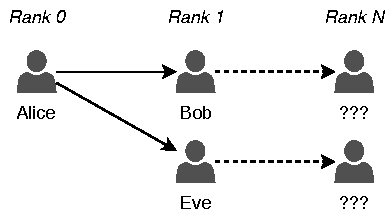
\includegraphics[width=1\linewidth]{fig3} 

}

\caption{Conceptual diagram of scholarly profiles and following others. Network propagation to rank N can be used to facilitate discovery of researchers and to build networks of researchers.}\label{fig:datcom-fig3}
\end{figure}

Using the \texttt{follows} property, Alice can propagate her feed deeper
into her network, as depicted in Figure \ref{fig:datcom-fig3}. More
specifically, Alice her own profile, rank zero in the network, extends
to the people she follows (i.e., Bob and Eve are rank one).
Subsequently, the profiles Bob and Eve follow are of rank three. By
using recursive functions to crawl the extended network to rank \(N\),
edges in the network are easily discovered despite the (potential) lack
of direct connections \citep{doi:10.2307/2786545}.

The \texttt{main} property can be used by a researcher to build a
personalized profile beyond the metadata. For example, Alice wants to
make sure that people who know the Dat link to her scholarly profile can
access her Curriculum Vitae, so she adds \texttt{/cv.pdf} as the
\texttt{main} to her scholarly profile. Whenever she submits a job
application, she can link to her versioned scholarly profile (e.g.,
\texttt{dat://b49...551+13}). Afterwards, she can keep updating her
profile whatever way she likes. She could even choose to host her
website on the decentralized Web by attaching a personal webpage with
\texttt{/index.html}. Because of the versioned link and the properties
of the Dat protocol, she can rest assured that the version she submitted
is the version the reviewing committee sees. Vice versa, whenever she
receives a versioned link to a scholarly profile, she can rest assured
it is what the researcher wanted her to see.

The \texttt{modules} property contains an array of versioned Dat links
to scholarly modules. What these scholarly modules are and how they are
shaped is explained in the next section. The \texttt{modules} property
differs from the \texttt{follows} property in that it can only contain
versioned Dat links, which serve as registrations of the outputs of the
researcher. Where a versioned link in the \texttt{follows} property is
regarded as a ``freeze follow,'' a versioned link in the
\texttt{modules} property is the registration and public communication
of the output. The versioned links also prevent duplicate entries of
outputs that are repeatedly updated. For example, a scholarly module
containing a theory could be registered repeatedly over the timespan of
several days or years. If the researcher would register non-versioned
links of the scholarly module, registration would not be specific and
the scholarly profile could contain duplicates. By including only
versioned links the registrations are specific and unique.

\subsection*{Scholarly modules}\label{scholarly-modules}

Scholarly research is composed of time-dependent pieces of information
(i.e., modules) that chronologically follow each other. For example,
predictions precede data and results, otherwise they become
postdictions. In a typical theory-testing research study, which adheres
to the framework of a modern empirical research cycle \citep{isbn:9789023228912}, we
can identify at least eight chronological modules of research outputs:
(1) theory, (2) predictions, (3) study design, (4) study materials, (5)
data, (6) code for analysis, (7) results, (8) discussion, and (9)
summary. Sometimes we might iterate between steps, such as adjusting a
theory due to insights gathered when formulating the predictions.
Continuously communicating these in the form of modules as they are
produced, by registering versioned references to Dat filesystems in a
scholarly profile as explained before, could fulfill the five functions
of a scholarly communication system and is unconstrained by the current
journal/article based system \citep[see also][]{doi:10.3390/publications6020021}.

These scholarly modules each live in their own filesystem, first on the
researcher's computer and when synchronized, on the Dat network. Hence,
researchers can interact with files on their own machine as they are
used to. The Dat network registers changes in the filesystem as soon as
it is activated. As such, researchers can initialize a Dat filesystem on
their computer and, for example, copy private information into the
filesystem, anonymize it and only then activate and synchronize it with
the Dat network (note: this does not require connection to the Internet,
but initialization of the protocol). The private information will then
not be available in the version history of the Dat filesystem.

Metadata for scholarly modules also consists of a generic
\texttt{dat.json} and a more specific \texttt{scholarly-metadata.json}.
The \texttt{dat.json} contains the title of the module, the description,
and its own Dat link. For example, Alice communicates the first module
on the network, where she proposes a theory; the \texttt{dat.json} file
for this module is


\begin{Shaded}
\begin{Highlighting}[]
\FunctionTok{\{}
  \DataTypeTok{"title"}\FunctionTok{:} \StringTok{"Mock Theory"}\FunctionTok{,}
  \DataTypeTok{"description"}\FunctionTok{:} \StringTok{"This is a mock theory but it could just as well be}
  \StringTok{a real one."}\FunctionTok{,}
  \DataTypeTok{"url"}\FunctionTok{:} \StringTok{"dat://dbf...d82"}
\FunctionTok{\}}
\end{Highlighting}
\end{Shaded}

Again, more specific metadata about the decentralized scholarly module
is added in \texttt{scholarly-metadata.json}. As the bare minimum, the
metadata for a scholarly module is initialized as

\begin{Shaded}
\begin{Highlighting}[]
\FunctionTok{\{}
  \DataTypeTok{"type"}\FunctionTok{:} \StringTok{"scholarly-module"}\FunctionTok{,}
  \DataTypeTok{"url"}\FunctionTok{:} \StringTok{"dat://dbf...d82"}\FunctionTok{,}
  \DataTypeTok{"authors"}\FunctionTok{:} \OtherTok{[}
    \StringTok{"dat://b49...551"}\OtherTok{,}
    \StringTok{"dat://167...a26"}
  \OtherTok{]}\FunctionTok{,}
  \DataTypeTok{"parents"}\FunctionTok{:} \OtherTok{[]}\FunctionTok{,}
  \DataTypeTok{"roots"}\FunctionTok{:} \OtherTok{[]}\FunctionTok{,}
  \DataTypeTok{"main"}\FunctionTok{:} \StringTok{"/theory.md"}
\FunctionTok{\}}
\end{Highlighting}
\end{Shaded}


These metadata indicate aspects that are essential in determining
contents and provenance of the module. First, we specify that it is a
scholarly module in the \texttt{type} property. Second, we specify its
own Dat \texttt{url} for reference purposes. Third, an array of Dat
links in the \texttt{authors} property links to scholarly profiles for
authorship. Subsequently, if the module is a direct consequence of a
previous registered module, we specify the Dat link of the preceding
module(s) in the \texttt{parents} property in the form of a versioned
Dat link. Tracing the parents' parents forms a chronology of findings,
leading ultimately to the \texttt{roots} property. In practice, the
\texttt{roots} property is inherited from the immediate parents. Because
the presented hypothetical module above is the first on the network, it
has no parents or roots. The \texttt{main} property specifies a single
landing page/file of the scholarly module. For a text based scholarly
module, \texttt{main} might be \texttt{/index.html} (or
\texttt{/theory.md} as it is here), whereas for a data module that could
be \texttt{/data.csv}. For more complex modules, a guidebook to navigate
the module could be included. The researcher can also store other
relevant assets in the Dat filesystem, such as converted files or
supporting files. For text based scholarly module, assets could include
figures; for data based scholarly modules assets could include
codebooks.

To register a module into the researcher's profile, the versioned Dat
link is included in the \texttt{modules} array on the profile. More
specifically, when the registration process is initiated, the Dat
filesystem is inspected for the latest version number, which is appended
to the Dat link before it is put in the \texttt{modules} property.
Specifically for Alice her theory, she was at version 19 when she wanted
to register it. This means that \texttt{dat://dbf...d82+19} is appended
to the \texttt{modules} array in her scholarly profile. All the users
who follow Alice get an update that she registered her theory, with a
versioned link that is unique and persistent, referring to exactly the
content Alice registered. Alice can keep updating her theory locally,
without it affecting what the people who follow her see, because it does
not affect version 19. When the module is registered, others can view
the most recent version of the Dat filesystem (e.g., theory) by removing
the version from the Dat link (or view any other synchronized version if
available from the network).

Figure \ref{fig:datcom-fig4} depicts how the scholarly modules relate to
each other (Panel B). The versioned, registered scholarly modules become
the parent and root links in subsequent child modules. For example, a
set of predictions link back to the theory they are distilled from; a
study design links back to the predictions it is planned to test and by
extension to the theory it is based on. Panel B in Figure
\ref{fig:datcom-fig4} conceptually depicts one contained empirical
research cycle registered in this way. The links between versioned
scholarly modules embeds the chronological nature of the research
process in its communication.

\begin{figure}

{\centering 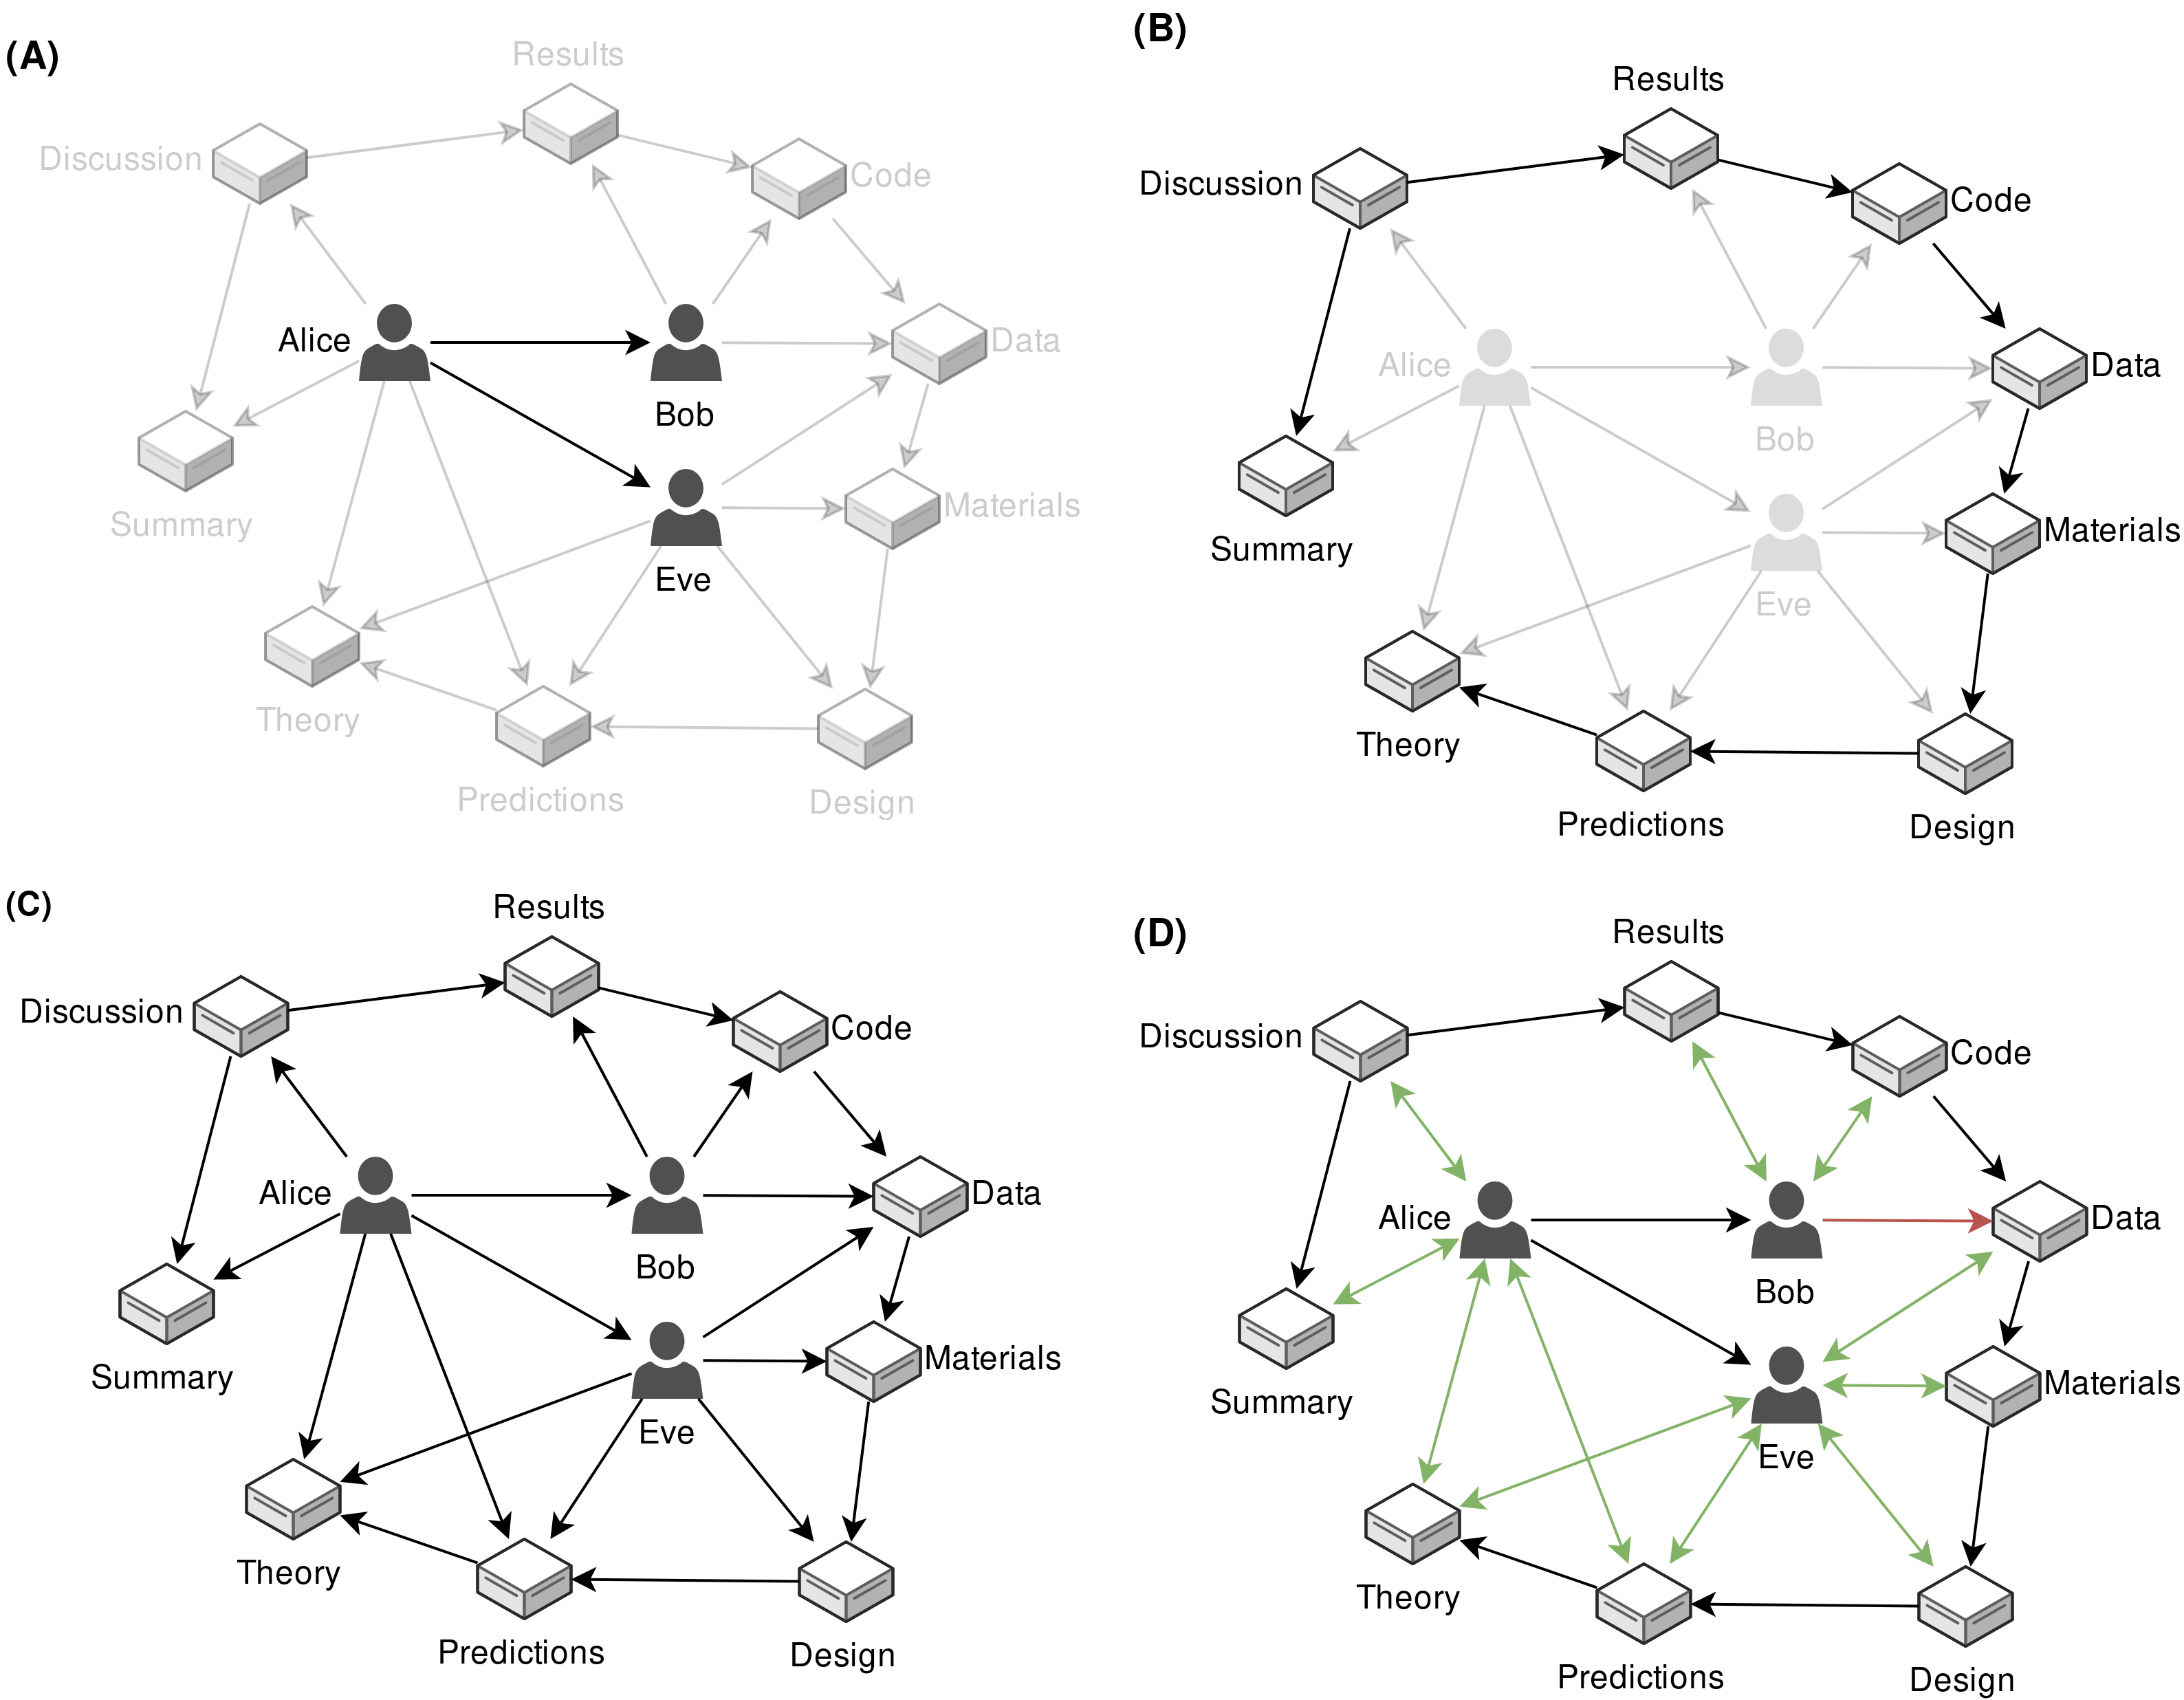
\includegraphics[width=1\linewidth]{fig4} 

}

\caption{Conceptual representations of how scholarly profiles relate to each other (Panel A), how scholarly modules relate to each other (Panel B), how scholarly profiles and modules create a network of scholarly activity in both researchers and research (Panel C), and how claims of authorship are verified if two-way or unverified if one-way (Panel D).}\label{fig:datcom-fig4}
\end{figure}

\subsection*{Verification}\label{verification}

In order to detect whether scholarly modules that a researcher claims to
have authored are indeed (partly) theirs, the scholarly module needs to
also assign the profile as author. For example, Alice and Eve claim to
have authored version 19 of the ``Theory'' module in their profiles
(Figure \ref{fig:datcom-fig4}, Panel C). Because a module can only be
edited by its author, we can inspect the scholarly module to corroborate
this. For verified authorship, the module should ascribe authorship to
Alice and Eve. To do this, we inspect \texttt{scholarly-metadata.json}
of the ``Theory'' module at the registered version (i.e., version 19).
If the versioned theory module also ascribes authorship to Alice or Eve,
we have two-way verification of authorship (Figure
\ref{fig:datcom-fig4}, Panel D). In other words, registered scholarly
modules must corroborate the authorship claims of the scholarly profiles
in order to become verified.

Unverified authorship can happen when a researcher incorrectly claims
authorship over a module or when a module ascribes authorship to a
researcher who does not claim it. In Figure \ref{fig:datcom-fig4} Panel
D, for example, Bob has claimed authorship of the data module, which is
not corroborated by the scholarly module. Unverified authorship of this
kind (i.e., where a researcher incorrectly claims authorship) is helpful
in preventing misrepresentation of previous work by that researcher.
Unverified authorship where a researcher is incorrectly ascribed
authorship can have various origins. A researcher might remove a
versioned module from their profile, effectively distancing themselves
from the module (similar to retracting the work but on a more individual
level). In a similar vein, it might also be that the author registered a
later version of the module in their profile and deleted the old version
(similar to a corrigendum). Note that the registration will still be
available in the history of the profile, because the history of a Dat
filesystem is append-only.

\subsection*{Prototype}\label{prototype}

In order to show that decentralized, modular scholarly communication is
not just a hypothetical exercise, a minimal working prototype is
available on the Dat network. This prototype is accessible using
\href{https://beakerbrowser.com}{Beaker Browser} at
\texttt{dat://b06...3dd/} (see Supporting File for full URL). This
prototype is currently only available within Beaker Browser because
specific Application Programmatic Interfaces (APIs) that directly
interface with the Dat protocol are not yet available in the most
commonly used Web browsers (e.g., Mozilla Firefox, Google Chrome).

The minimal working prototype ingests a network of decentralized
scholarly modules and profiles. More specifically, it ingests all
content to rank \(N\) of the network, using
\href{https://github.com/beakerbrowser/webdb}{\texttt{webdb}}.
\texttt{webdb} collects the scholarly metadata from each scholarly
module and scholarly profile and consolidates these disparate pieces of
information into a local database. This database can be considered
temporary; the original information still has its primary origin in the
disparate scholarly modules and scholarly profiles that live on the Dat
network. As such, the same database can be reconstructed at any time
without any issues, assuming the modules are still available. Figure
\ref{fig:datcom-fig5} presents a screenshot of the prototype, which
looks like any other webpage to the user but does not have a centralized
server providing the content. Note also the link at the bottom
showcasing the versioned link to the analysis file.

\begin{figure}

{\centering 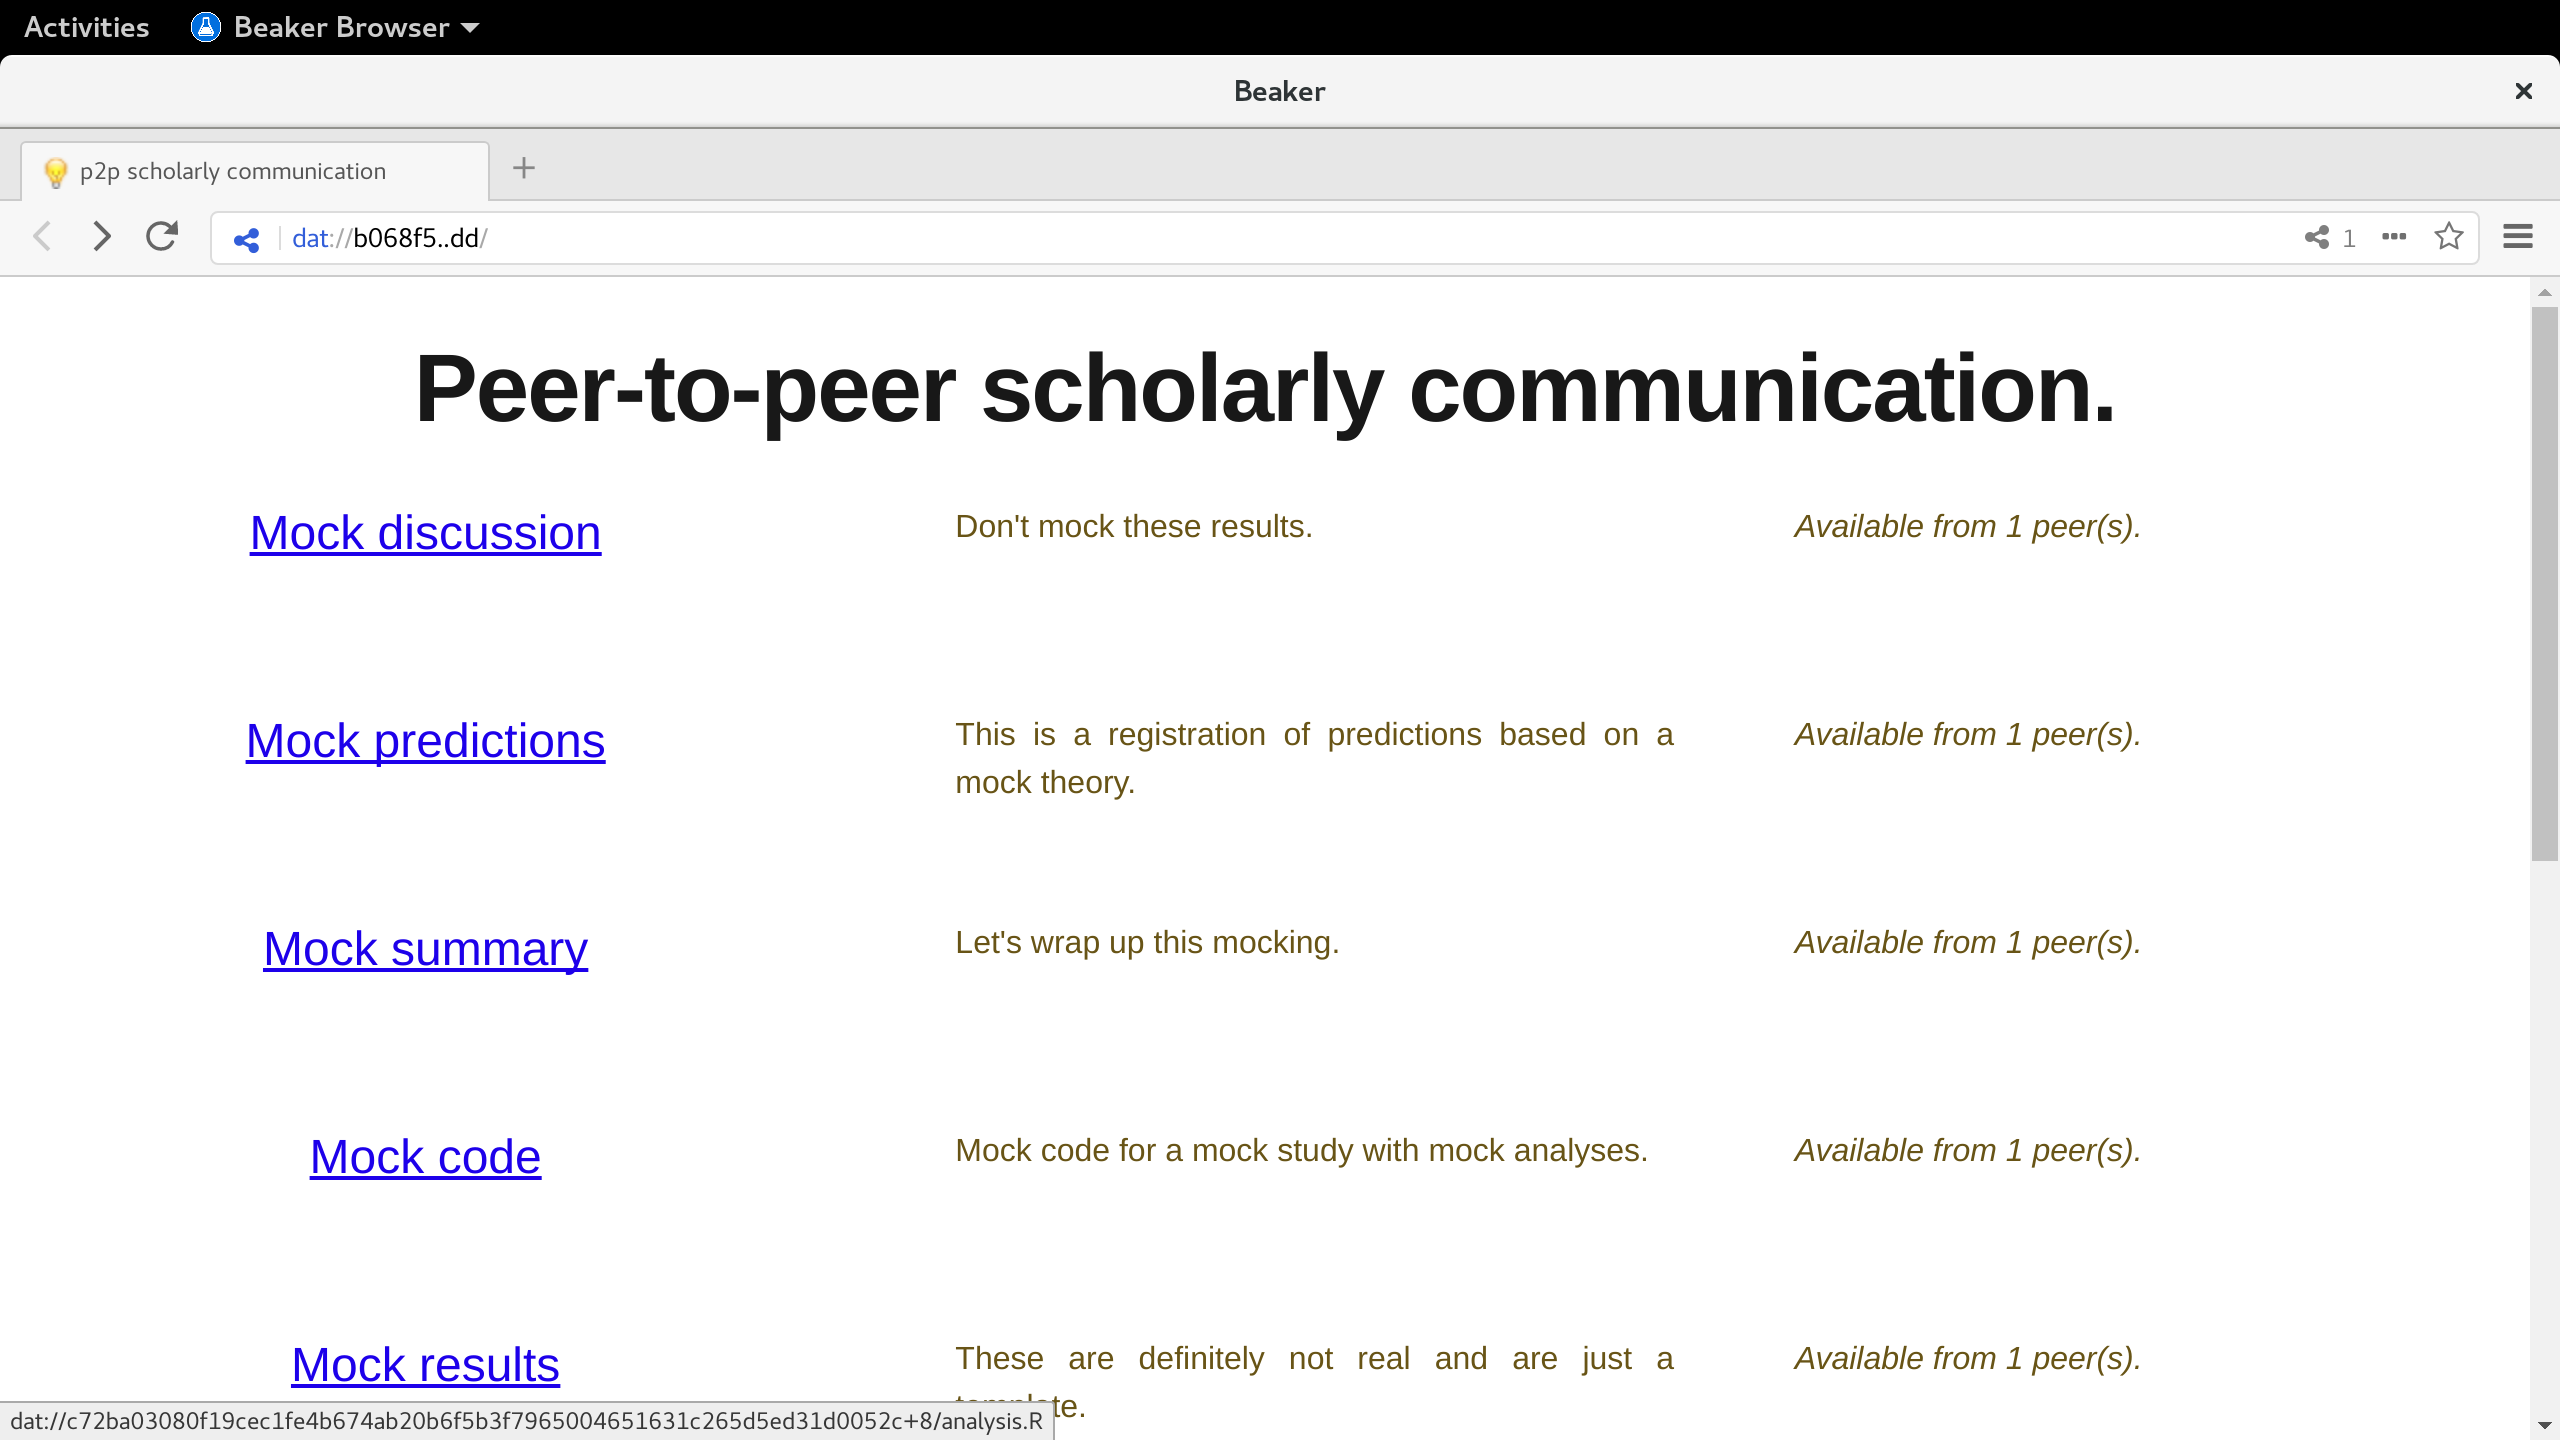
\includegraphics[width=1\linewidth]{fig5} 

}

\caption{Screencap of the minimal prototype of decentralized scholarly communication. The prototype resembles a regular webpage on the userside, but on the backend it runs entirely on Dat filesystems that live on a decentralized network.}\label{fig:datcom-fig5}
\end{figure}

Procedurally, the prototype takes Alice's scholarly profile as starting
point, subsequently ingesting the network presented in Figure
\ref{fig:datcom-fig4}. By doing so, we get a one-on-one replication of
Alice's perspective (regardless of whether we are Alice or not). As
such, Alice's Dat link serves as the starting point (rank zero). The
metadata contained in her profile is ingested into our local database.
Subsequently, the links in her profile to other scholarly modules (or
profiles) are ingested into the database (rank one), and the links they
have (rank two), and so on (to rank \(N\)). The following JavaScript
code produces this local database for Alice specifically
(\texttt{dat://b49...551}) but can be replaced with Bob's, Eve's, or
anyone else's scholarly profile to receive their personal network.


\begin{Shaded}
\begin{Highlighting}[]
\CommentTok{// npm install -g @beaker/webdb}
\KeywordTok{const}\NormalTok{ WebDB }\OperatorTok{=} \AttributeTok{require}\NormalTok{(}\StringTok{'@beaker/webdb'}\NormalTok{)}

\KeywordTok{let}\NormalTok{ webdb }\OperatorTok{=} \KeywordTok{new} \AttributeTok{WebDB}\NormalTok{(}\StringTok{'view'}\NormalTok{)}

\VariableTok{webdb}\NormalTok{.}\AttributeTok{define}\NormalTok{(}\StringTok{'modules'}\OperatorTok{,} \OperatorTok{\{}
    \DataTypeTok{filePattern}\OperatorTok{:}\NormalTok{ [  }\StringTok{'/scholarly-metadata.json'}\NormalTok{  ]}\OperatorTok{,}
    \DataTypeTok{index}\OperatorTok{:}\NormalTok{ [ }\StringTok{'type'}\OperatorTok{,} \StringTok{'authors'}\OperatorTok{,} \StringTok{'parents'}\OperatorTok{,} \StringTok{'root'}\OperatorTok{,}
     \StringTok{'main'}\OperatorTok{,} \StringTok{'follows'}\OperatorTok{,} \StringTok{'modules'}\NormalTok{ ]}
\OperatorTok{\}}\NormalTok{)}

\NormalTok{async }\KeywordTok{function} \AttributeTok{ingestPortal}\NormalTok{ (url) }\OperatorTok{\{}
\NormalTok{  await }\VariableTok{webdb}\NormalTok{.}\AttributeTok{open}\NormalTok{()}

  \KeywordTok{let}\NormalTok{ archive }\OperatorTok{=} \KeywordTok{new} \AttributeTok{DatArchive}\NormalTok{(url)}
\NormalTok{  await }\VariableTok{webdb}\NormalTok{.}\AttributeTok{indexArchive}\NormalTok{(url)}
  
  \KeywordTok{let}\NormalTok{ scholRaw }\OperatorTok{=}\NormalTok{ await }\VariableTok{archive}\NormalTok{.}\AttributeTok{readFile}\NormalTok{(}
    \StringTok{'/scholarly-metadata.json'}\NormalTok{)}
  
  \KeywordTok{let}\NormalTok{ scholParsed }\OperatorTok{=}\NormalTok{ await }\VariableTok{JSON}\NormalTok{.}\AttributeTok{parse}\NormalTok{(}
\NormalTok{    scholRaw)}
  
  \ControlFlowTok{if}\NormalTok{ (}\VariableTok{scholParsed}\NormalTok{.}\AttributeTok{type} \OperatorTok{===} \StringTok{'scholarly-profile'}\NormalTok{) }\OperatorTok{\{}
    \VariableTok{console}\NormalTok{.}\AttributeTok{log}\NormalTok{(scholParsed)}
    \VariableTok{scholParsed}\NormalTok{.}\VariableTok{follows}\NormalTok{.}\AttributeTok{concat}\NormalTok{(}
      \VariableTok{scholParsed}\NormalTok{.}\AttributeTok{modules}\NormalTok{).}\AttributeTok{forEach}\NormalTok{((val) }\OperatorTok{=>} \OperatorTok{\{}
      \AttributeTok{ingestPortal}\NormalTok{(val)}
    \OperatorTok{\}}\NormalTok{)}
  \OperatorTok{\}}
\OperatorTok{\}}

\AttributeTok{ingestPortal}\NormalTok{(}\StringTok{"dat://b49...551"}\NormalTok{)}
\end{Highlighting}
\end{Shaded}

The presented prototype provides a portal to the information contained
in the modules, but is not the sole portal to access that information.
Because the modules live on a decentralized network and are
open-by-design, anyone may build a portal to view that information
(Figure \ref{fig:datcom-fig6} presents a mockup of an additional
interface). As such, this is not a proposal for a platform but for
infrastructure. The difference between platforms and infrastructure is
vital in light of ownership and responsibility of communicated content
and the moderation of that content. As opposed to centralized services
that carry the legal burden and therefore moderate its platform, this
type of infrastructure does not take such a role and merely aims to
facilitate the individual. As a consequence, the legal burden remains
with the individual. Moreover, platforms require people to go to one
place (e.g., you cannot view content of ResearchGate on Academia.edu or
Elsevier's content on Wiley's webpage); this infrastructure would give
the potential for various types of usage to take place on the same type
of infrastructure.

\begin{figure}
\centering
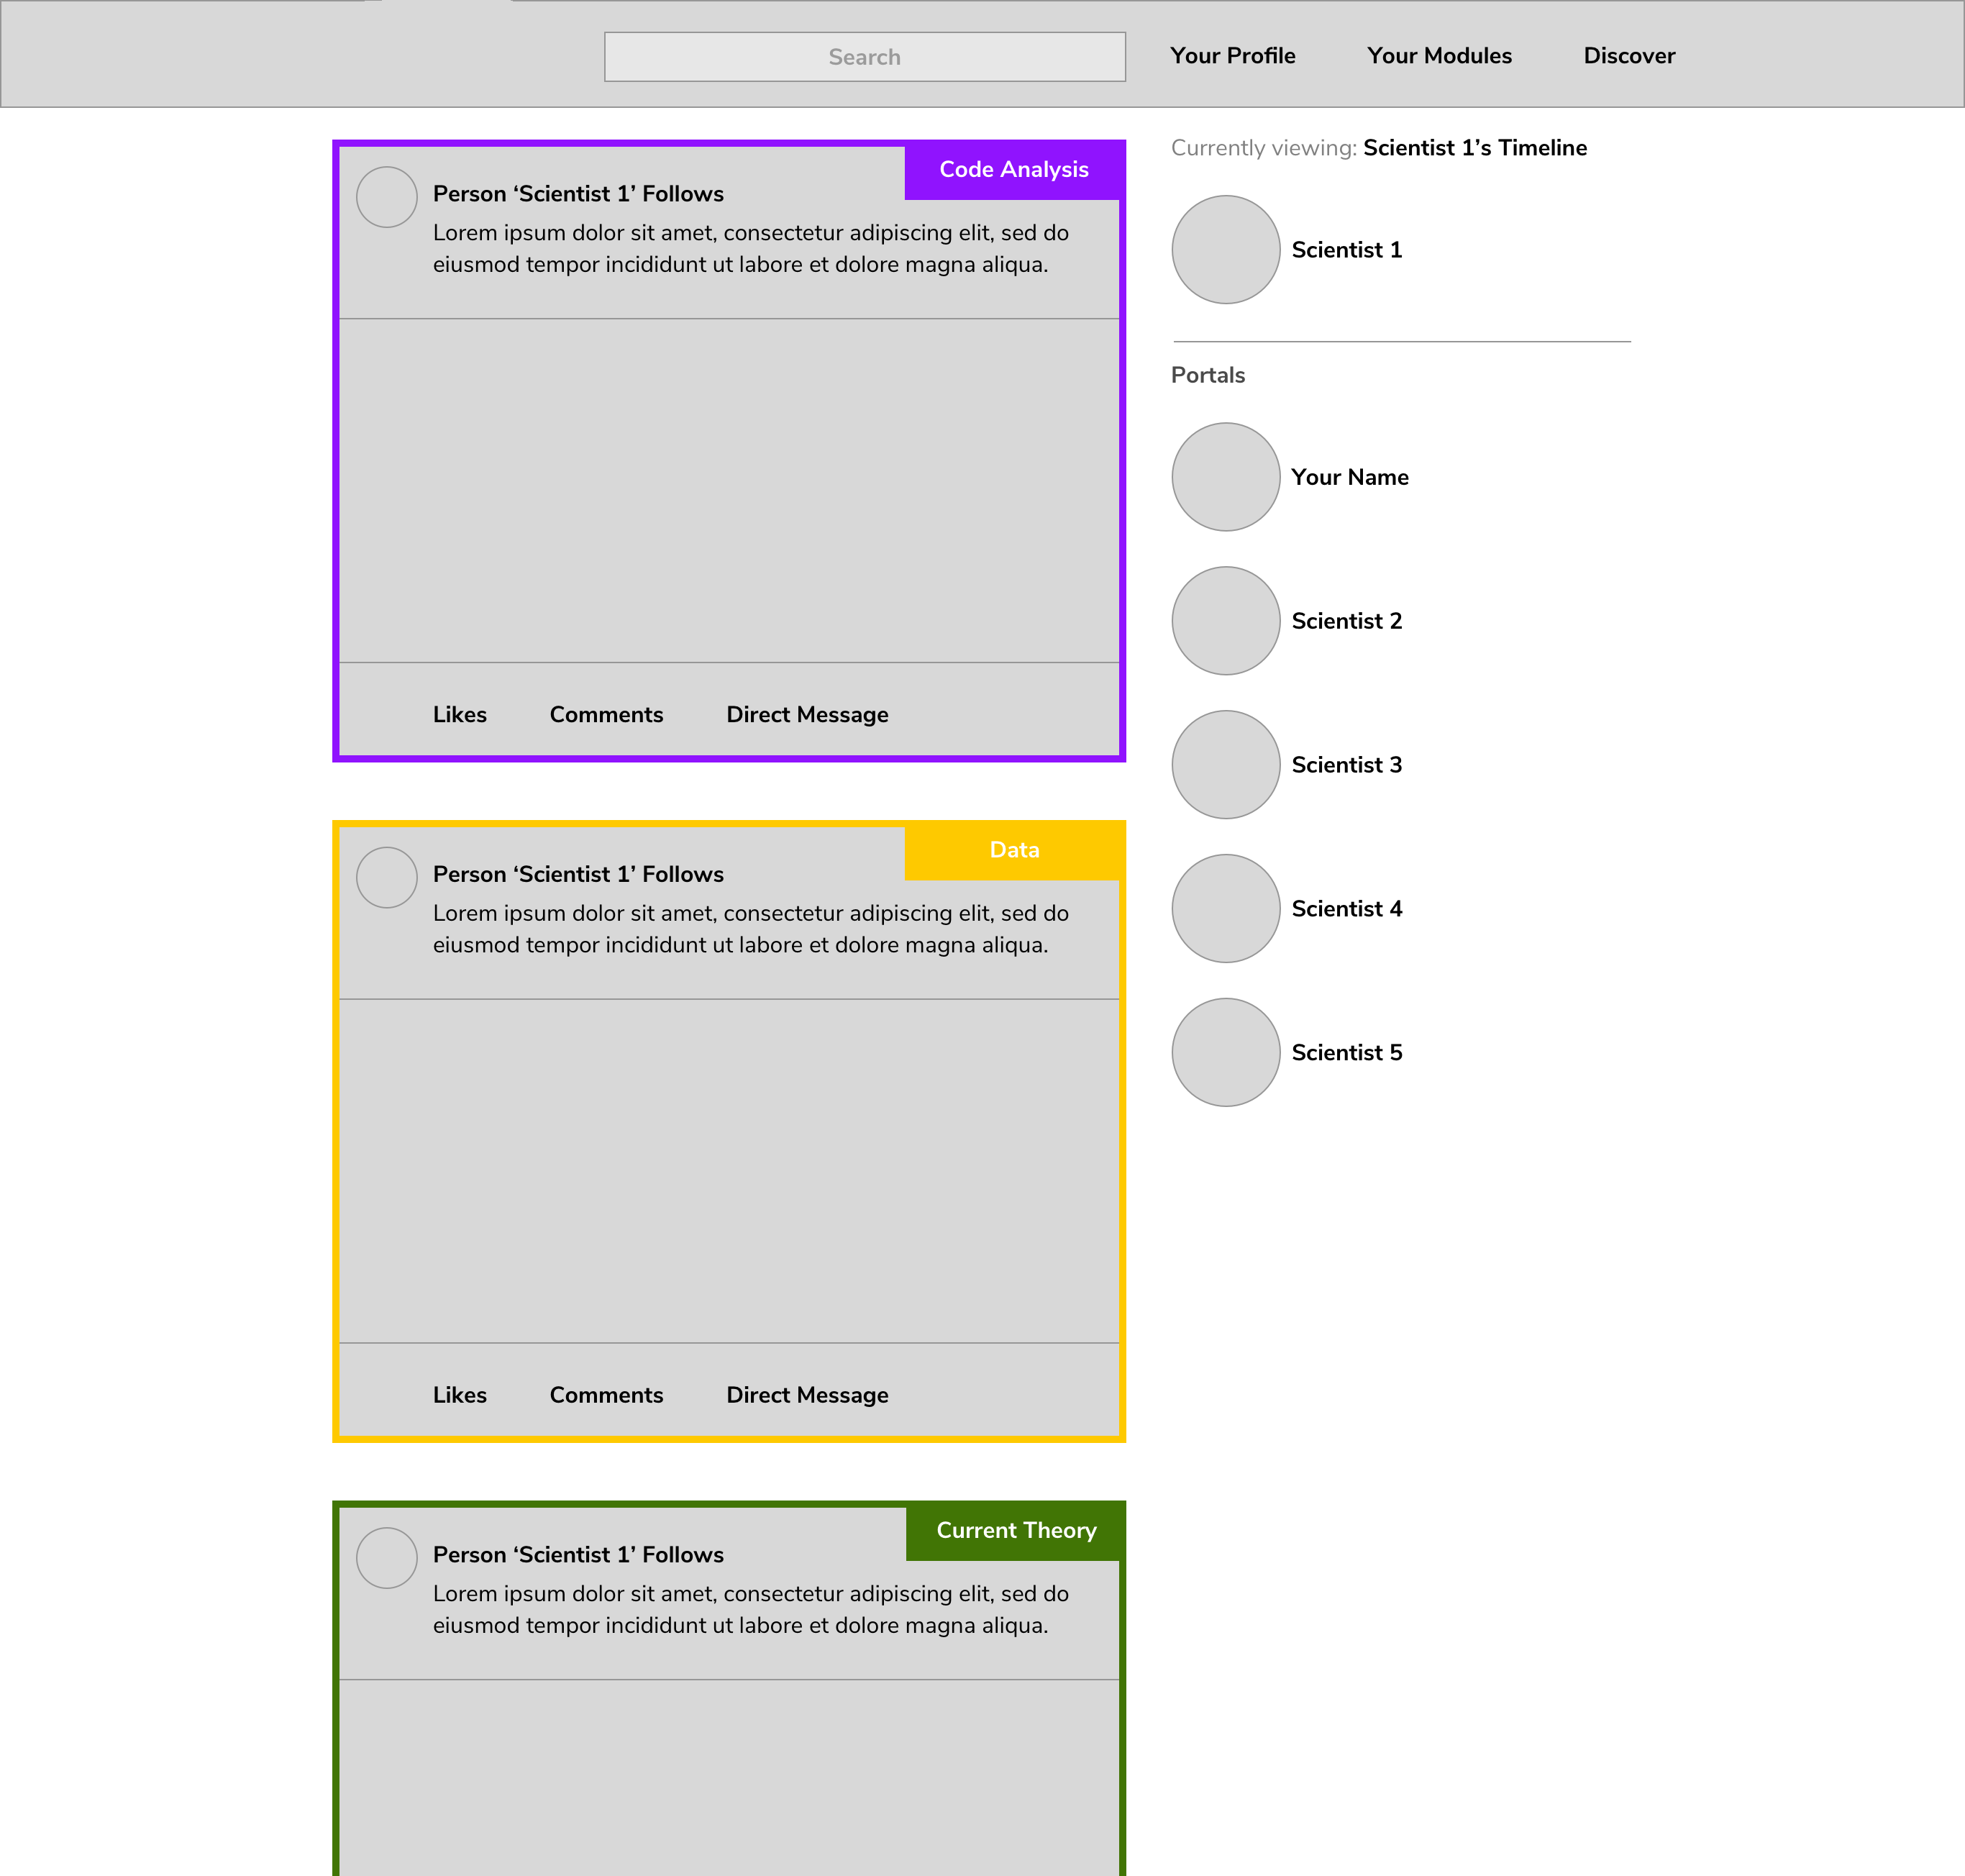
\includegraphics{mockup-1a.png}
\caption{Mockup design of an additional interface for the proposed
scholarly communication infrastructure. Made by Rebecca Lam, reused
under CC-BY 4.0 license.}
\label{fig:datcom-fig6}
\end{figure}

\section*{Discussion}

The proposed design for decentralized, verified, provenance based modular communication on the Dat protocol fulfills a wide conceptualization of the functions of a scholarly communications system from library and information sciences \citep{roosendaal1998,doi:10.1045/september2004-vandesompel}. Due to more modular and continuous communication, it is more difficult to selectively register results when the preceding steps have publicly been registered already. Moreover, time of communication is decided by the researcher, making it more feasible for researchers to communicate their research efforts without biases introduced at the journal level. Certification of results is improved by embedding the chronology of the empirical research cycle in the communication process itself and making peer-to-peer discussion constructive and less obstructed by hindsight bias \citep{doi:10.1037/1089-2680.2.2.175}. Unfettered awareness of research is facilitated by using an open-by-design infrastructure that is the peer-to-peer Dat protocol. Moreover, because all content is open-by-design and independent of service platforms, text- and data-mining may be applied freely without technical restrictions by service providers. The removal of these technical and service restrictions may facilitate innovations in discovery of content and the potential for new business models to come into existence. Based on the links between scholarly modules, the arising network structure can be used to help evaluate networks of research(ers) instead of counting publications and citations \citep{doi:10.3390/publications6020021}.
Archival is facilitated by making it trivially easy to create local copies of large sets of content, facilitating the Lots Of Copies Keeps Stuff Safe \citep[LOCKSS;][]{doi:10.1045/june2001-reich,doi:10.1103/physreve.95.022313} principle to be more widely used than just approved organizations. Moreover, with append-only registers, the provenance of content can also be archived more readily than it is now. These functions also apply to non-empirical research that requires provenance of information (e.g., qualitative studies).

By producing scholarly content on a decentralized infrastructure, diversity of how research is consumed and discovered can be facilitated. Currently, content lives on the webserver of the publisher and is often solely served at the publisher's webpage due to copyright restrictions \citep[except for open access articles;][]{doi:10.7717/peerj.4375}. If the design of the publisher's webpage does not suit the user's needs \citep[e.g., due to red color blindness affecting approximately 1 in 20 males and 1 in 100 females;][]{doi:10.1016/j.gendis.2015.02.006}, there is relatively little a user can do. Moreover, service providers that are not the rightsholder (i.e., publisher) now cannot fulfill that need for users. By making all content open, building on content is possible by anyone who feels like it. For example, someone can build a portal that automatically shows content with color shifting for people who have red (or other types of) color blindness. Building and upgrading automated translation services are another way of improving accessibility (e.g., \href{http://translexy.com/}{translexy.com/}), which is currently restricted due to copyright. 
Other examples of diverse ways of consuming or discovering research might include text-based comparisons of modules to build recommender algorithms that provide contrasting and corroborating views to users. Stimulating diversity in how to consume and discover content is key to making scholarly research accessible to as many people and in order to attempt to keep some pace with the tremendous amount of information published each year (\href{https://api.crossref.org/works?filter=type:journal-article,from-pub-date:2017,until-pub-date:2017\&rows=0}{\textgreater{}3
million articles in 2017}). As such, we have collectively passed the point of being able to comprehend the relevant information and should no longer strive to eliminate all uncertainty in knowing but find ways to deal with that uncertainty better \citep{isbn:9781786635471}. As such, alternatives in consuming, discovering, and learning about knowledge are a necessity. Open Knowledge Maps is an existing example of innovative discovery mechanisms based on openly licensed and machine-readable content \citep{doi:10.12685/027.7-4-2-157}. There would be more smaller pieces of information in the scholarly modules approach, which is counterbalanced by the network structure and lack of technical restrictions to build tools to digest that information --- this may make those larger amounts of smaller units (i.e., modules) more digestible than the smaller volume of larger units (i.e., articles). 

The proposed design is only the first in a multi-layer infrastructure that would need to be developed moving forward. Currently, I only provide a model on the container format for how to store metadata for modules --- not how the data is stored in the module itself or how the individual could go about doing so. Moreover, how could reviews be structured to fit in such modules? 
As such, the next layer to the proposed infrastructure would require further specification of how contents are stored. For example, for text-based modules, what file formats should be the standard or allowed? It would be unfeasible to allow any file format due to readability into the future (e.g., Word 2003 files are likely to be problematic) and issues could exacerbate if software becomes more proprietary and research uses more types of software. Standards similar to current publications could prove worthwhile for text (i.e., JATS XML), but impractical to non-technical users. As such, does the original file need to be in JATS XML when it can also easily be converted? \citep[e.g., Markdown to JATS XML;][]{jatdown} Other specifications for data, code, materials would also be needed moving forward (e.g., no proprietary binary files such as SPSS data files). In order to make those standards practical to individuals not privy to the technical details, the next infrastructure layer would be building user-facing applications that interface with the Dat protocol and take the requirements into account. These would then do the heavy lifting for the users, guiding them through potential conversion processes. An example of a rich editing environment that takes the machine readability of scholarly text to the next level, and makes this relatively easy to the end-user, is Dokie.li \citep[which writes to HTML;][]{dokieli}. This editing environment provides a What You See Is What You Get (WYSIWYG) editor, while at the same time providing semantic enrichments to the text (e.g., discerning between positive, negative, corroborating, or other forms of citations).

New infrastructure layers could provide a much needed upgrade to the security of scholarly communication. Many of the scholarly publisher's websites do not use an appropriate level of security in transferring information to and from the user. More specifically, only 26\% of all scholarly publishers use HTTPS \citep{https-hartgerink}. Science Magazine only recently implemented HTTPS, and Sage Publications is one example that still has not. This means that any information transferred to or from the user can be grabbed by anyone in the physical proximity of that person (amongst other scenarios) --- including usernames and passwords. In other words, publisher's lack of up-to-date security practices put the user at risk, but also the publisher. Some publishers for example complained about Sci-Hub, alleging that it illegally retrieved articles by phishing researcher's credentials. A lack of HTTPS would facilitate the illegal retrieval of user credentials, hence those publishers would ironically facilitate the kinds of activities they say are illegal \citep{doi:10.1126/science.aaf5664}. Beyond the potential of missed revenue for pay-to-access publishers, security negligence is worrisome because the accuracy of scholarly content is at risk. Man-in-the-middle attacks, where a middleman inserts themselves between the user and the server, can surreptitiously distort content, with practical effects for scientific practice (e.g., changing author names) and real life effects for professions using results for their jobs (e.g., milligram dosages replaced by gram dosages). By building a scholarly communication infrastructure on top of the Dat protocol, all communications are encrypted in transit from one end to the other by default. For the format of communications, scholarly publishers may currently be unknowing distributors of malware in their PDFs distributed to (paying) readers. More specifically, an estimated .3-2\% of scholarly PDFs contain malware \citep{doi:10.3233/978-1-61499-744-3-107}, although the types of malware remain ill specified. By implementing scholarly modules that are converted on the user's system (e.g., JATS XML, HTML, Markdown), the attack vector on readers of the scholarly literature can be reduced by moving away from server-side generated PDFs, which potentially contain clandestine malware.

\subsection{Limitations}

One of the major points of debate may be that the scholarly modules are
chronologically ordered only (both internally and externally). As such,
the temporal distance between two actions within a scholarly module or
between two scholarly modules is unknown. Within a scholarly module and
Dat filesystem, chronological append-only actions are more reliable to
register from a technical perspective than time-based append-only
registers. This has its origin in the fact that creation-,
modification-, and last opened times can technically be altered by
willing users (see for example
\href{https://superuser.com/questions/504829}{superuser.com/questions/504829}).
If timestamps are altered, people can fabricate records that seem
genuine and chronological, but are not --- undermining the whole point
of immutable append-only registers. Hardcoded timestamps in the
scholarly metadata would be an even greater risk due to the potential
for direct modification (i.e., it would only require editing the
\texttt{scholarly-metadata.json} file in a text editor). The external
ordering, that is the chronology of scholarly modules, might be gamed as
well. Consider the scenario where a predictions module at version 12 is
said to be the parent of a design module at version 26 but does not
exist yet at the time of registration for the design module. An
individual with malicious intentions might do this and retroactively
fabricate the parent predictions. So, despite a specific, persistent,
and unique parent Dat link being provided, the chronology could be
undermined, which in turn threatens the provenance of information. It
would require some effort from said researcher to subsequently ensure
that the referenced Dat link contains the postdictions, but it is
possible to fake predictions in this manner (but this is a bigger
problem in the current system). Other mechanisms could be put in place
to verify the existence of parent links at the time of registration
(which is technically feasible but would require additional bodies of
trust) or to technically investigate for filler actions in a Dat
filesystems when artificially high version numbers are registered.

Despite the potential of building an open-by-design scholarly
infrastructure on top of the Dat protocol, there are also domains where
advances need to be made. Until those advances are made, widespread use
in the form of a scholarly communication system remains impractical and
premature. These developments can occur asynchronously of the further
development of this scholarly communication infrastructure. Amongst
others, these domains include technical aspects and implementations of
the Dat protocol itself, implementations of APIs built on top of it,
legal exploration of intellectual property on a peer-to-peer network,
privacy issues due to high difficulty of removing content permanently
once communicated, the usability of the proposed scholarly
infrastructure, and how to store information in the modules that is
machine readable but also easy-to-use for individuals.

The Dat protocol is functional, but is currently limited to NodeJS and
single-user write access. Because it is currently only available in
NodeJS, portability of the protocol is currently restricted to
JavaScript environments. An experimental implementation of the Dat
protocol is currently being built \href{https://github.com/datrs}{in
Rust}, which would greatly improve availability of the protocol to other
environments. Moreover, by being restricted to single-user write access,
Dat archives are not really portable across machines or users, although
work on multi-user write (i.e., multiple devices or users)
\href{https://github.com/mafintosh/hyperdb}{has recently been released}.
Other APIs built on top of the Dat protocol that are essential to
building a proposed infrastructure, such as \texttt{webdb}, also need to
be further refined in order to make them worthwhile. For example,
\texttt{webdb} currently does not index versioned Dat links but simply
the most recent versions. As such, the indexing of versioned references
is problematic at the moment, but can be readily tackled with further
development. If these and other developments continue, the benefits of
the protocol will mature, may become readily available to individuals
from within their standard browser, and become more practical to
collaborate on. Considering this, the proposed design is imperfect but
timely, allowing for community driven iterations into something more
refined as implementations of the Dat protocol are also refined and may
become more widely used.

Despite the Dat protocol's peer-to-peer nature, intellectual property
laws still ascribe copyright upon creation and do not allow copying of
content except when explicitly permitted through non-restrictive
licenses by authors \citep{isbn:9781400851911}. As such, intellectual property laws
could be used to hamper widespread copying when licensing is neglected
by authors. Legal uncertainty here might give rise to a chilling effect
to use the Dat protocol to share scholarly information. Moreover, it
seems virtually impossible to issue takedown notices for (retroactively
deemed) illicit content on the Dat protocol without removing all peer
copies on the network. As a result of this, social perception of the Dat
protocol might turn negative if high-profile cases of illicit or illegal
sharing occur (regardless of whether that is scholarly information or
something else). However, just as the Web requires local copies in cache
to function and which lawmakers made legal relatively quickly when the
Web was becoming widespread, the wider implementation of peer-to-peer
protocols to share content might also require reforms to allow for more
permissive copying of original content shared on the network.
Regardless, legal issues need to be thought about beforehand and users
should be made aware that they carry responsibility for their shared
content. Given its inherent open and unrestricted sharing design, it
would make sense to use non-restrictive licenses on the scholarly
modules by default to prevent these legal issues for researchers wanting
to reuse and build on scholarly modules.

Similarly, we need to take seriously the issue that information on the
network, once copied by a peer or multiple peers, is increasingly
unlikely to be uncommunicated. The implications of this in light of
privacy legislations, ethical ramifications, and general negative
effects should not be underestimated. Because a Dat filesystem has a
stable public key and stores versions, the content remains available
even if the content is deleted from the filesystem. That is, users could
go to an older version and still find the file that was deleted. The
only way to truly undo the availability of that information is to remove
all existing copies. Hence, it is worthwhile to ask the question whether
scholarly research that is based on personal data should ever be
conducted on the individual level data or whether this should be done on
higher level summaries of relations between variables (e.g., covariance
matrices). How these summaries can be verified, would remain an issue to
tackle. Conversely, the limitation with respect to privacy is also a
benefit with regards to censorship, where information would also be much
harder to censure \citep[in stark contrast to publishers that might be
pressured by governments;][]{guardian-cup}. Moreover, we might start
thinking about the ownership of data in research. In the case of human
subjects research, researchers now collect data and store it, but we
might consider decentralized data collection where human participants
produce their own data locally and simply permit a researcher to ingest
that into an analysis process (creating throwaway databases themselves
with \texttt{webdb} for example). This would in turn return ownership to
the participant and benefit transparency of data generated.

Bandwidth and persistent peers on the Dat protocol are highly correlated
issues that are key to a usable decentralized infrastructure. When there
are few peers on the network, information redundancy is low, content
attrition is (potentially) high, and bandwidth will be limited.
Subsequently, maximum data transfer of 40KB/s may be possible when few
peers with restricted bandwidth are available and are farther removed on
the physical network. Vice versa, in the most optimal scenario data
transfer could reach the maximum of the infrastructure between peers
(e.g., 1GB/s on peers located on an intranet). Considering that
replicating Dat filesystems is relatively easy given storage space, it
could be done by individuals, and (university) libraries seem
particularly qualified and motivated candidates for persistent hosting
of content on the Dat network. These organizations often have
substantial server infrastructure available, would facilitate high data
transfer speeds, and also have a vested interested in preserving
scholarly content. With over 400 research libraries in Europe and over
\href{http://db.aflia.net/list/?q=6\&m=n}{900 academic libraries in
Africa} alone, bandwidth and redundancy of scholarly content could be
addressed if sufficient libraries participate in rehosting content.
Moreover, the peer-to-peer nature would also allow for researchers to
keep accessing content in the same way when the content is rehosted on
the intranet and the wider connection has service interruptions.

\hypertarget{conclusion}{%
\subsection{Conclusion}\label{conclusion}}

The semi-technical proposal for verified, modular, and provenance based
scholarly infrastructure on the Dat protocol synthesizes meta-research,
technical developments of new Web protocols, real-life issues in a lack
of diversity for consuming scholarly research, and library and
information science's perspectives on the five functions scholarly
communication is supposed to fulfill. With this initial proposal a
scholarly commons seems feasible. The proposal provides a more complete
and less biased register of information than the current article-based
system. Moreover, it facilitates more constructive certification
discussions and allows anyone with access to the Internet to
participate. It also provides archival supportive of the distribution,
which anyone may meaningfully contribute to if they have the physical
means. This proposal also may provide new ways of evaluating, consuming,
and discovering research. The decentralized nature of the Dat protocol
requires less trust to be put in institutions to maintain key data
stores that are the fundament to any infrastructure and replaces it with
widespread distribution of that information. However, technological,
legal, and social developments need to occur asynchronously to make this
a reality.

%%%%%%%%%%%%%%%%%%%%%%%%%%%%%%%%%%%%%%%%%%
%%%%%%%%%%%%%%%%%%%%%%%%%%%%%%%%%%%%%%%%%%
\vspace{6pt} 

%% optional
\supplementary{S1 File. Overview of original Dat links corresponding to shortened
links:
\url{https://github.com/chartgerink/2018dat-com/raw/master/assets/mock-modules-overview.ods}.
}

% Only for the journal Methods and Protocols:
% If you wish to submit a video article, please do so with any other supplementary material.
% \supplementary{The following are available at \linksupplementary{s1}, Figure S1: title, Table S1: title, Video S1: title. A supporting video article is available at doi: link.}

%%%%%%%%%%%%%%%%%%%%%%%%%%%%%%%%%%%%%%%%%%
\authorcontributions{Conceptualization, CHJH; software, CHJH; investigation, CHJH; resources, CHJH; writing—original draft preparation, CHJH; writing—review and editing, CHJH; visualization, CHJH; project administration, CHJH; funding acquisition, CHJH}

%%%%%%%%%%%%%%%%%%%%%%%%%%%%%%%%%%%%%%%%%%
\funding{This research was partly funded by the Mozilla Foundation.}

%%%%%%%%%%%%%%%%%%%%%%%%%%%%%%%%%%%%%%%%%%
\acknowledgments{The author thanks everyone who has helped incubate this idea in the discussions over the last two years.}

%%%%%%%%%%%%%%%%%%%%%%%%%%%%%%%%%%%%%%%%%%
\conflictsofinterest{The author declares no conflict of interest.} 

%%%%%%%%%%%%%%%%%%%%%%%%%%%%%%%%%%%%%%%%%%
%% optional
%%%%%%%%%%%%%%%%%%%%%%%%%%%%%%%%%%%%%%%%%%
%% optional
\appendixtitles{no} %Leave argument "no" if all appendix headings stay EMPTY (then no dot is printed after "Appendix A"). If the appendix sections contain a heading then change the argument to "yes".
% \appendixsections{multiple} %Leave argument "multiple" if there are multiple sections. Then a counter is printed ("Appendix A"). If there is only one appendix section then change the argument to "one" and no counter is printed ("Appendix").

%\externalbibliography{yes}
\bibliography{shared-logs}

%%%%%%%%%%%%%%%%%%%%%%%%%%%%%%%%%%%%%%%%%%
\end{document}